% - PER STILARE QUESTO DOCUMENTO VANNO INSERITI I DATI.
% - VISTO CHE IL FILE È LUNGO ED INTRICATO PER SEMPLIFICARE HO MESSO DEI COMMENTI
% - CHE INDICANO I PUNTI DOVE INSERIRE LE INFORMAZIONI CHE MANCANO.
% - INSERISCILI IN CORRISPONDENZA DEI COMMENTI:

% - "INSERT TITOLO"
% - "INSERT USO"
% - "INSERT DATA"
% - "INSERT DESCRIZIONE"
% - "INSERT INFORMAZIONI INCONTRO"
% - "INSERT DOMANDE E RISPOSTE" (intanto lo strutturiamo così, con domande e rispose, se servono altri tipi di struttura cambieremo)

% - "INSERT TITOLO" (verosimilmente sarà una cosa tipo "Verbale Esterno/Interno del xx/yy")


\makeatletter
\newcommand\HUGE{\@setfontsize\Huge{40}{50}}
\makeatother    
 
\newcommand{\Titolo}{Neuradillo}

\newcommand{\Gruppo}{Giovanni Sorice \\
Francesco Corti}

\newcommand{\Versione}{1.0.0}

\newcommand{\Redazione}{}




\documentclass[a4paper, oneside, openany]{article}
\usepackage{titling}
\usepackage{graphbox}
\usepackage{amsmath , amssymb , amsthm}
\usepackage{comment} 
% permette di modificare i margini
\usepackage[top=3.1cm, bottom=3.1cm, left=2.2cm, right=2.2cm]{geometry}

\usepackage{lastpage} %info sul # dell'ultima pagina del documento
\usepackage{fancyhdr} %per modificare dimensioni,margini, intestazioni e righe a piè di pagina
\fancypagestyle{plain}{
  % cancella tutti i campi di intestazione e piè di pagina
  \fancyhf{}
  
  %\lfoot{ %piè di pagina
   %{\Titolo} \ - \textit{{\Gruppo}}
  %}
  \rfoot{Page \thepage{} of \pageref{LastPage}} %es: pag: 4 di 10

  %linea orizzontale alle posizioni top e bottom della pagina
  \renewcommand{\headrulewidth}{0.2	pt}  
  \renewcommand{\footrulewidth}{0.2pt}
}
\pagestyle{plain}

%Comando Spazio
\newcommand{\Spazio}{\mbox{} \\ \mbox{} \\ }  


%\usepackage{calc} %introduce la notazione infissa per le op. aritmetiche interne a LaTeX

\usepackage[utf8]{inputenc}
\usepackage[T1]{fontenc}
\usepackage[english]{babel} %il documento è in italiano
%\usepackage{textcomp} %The pack­age sup­ports the Text Com­pan­ion fonts, which pro­vide many text sym­bols
%(such as baht, bul­let, copy­right, mu­si­cal­note, onequar­ter, sec­tion, and yen), in the TS1 en­cod­ing.

\usepackage{graphicx}       %permette di inserire delle immagini
\usepackage{caption}        %numerazione figure e loro descrizione testuale
\usepackage{subcaption}     %sottofigure numerabili
\usepackage{float}  %permette di inserire un # qualsiasi di figure fluttuanti
\usepackage{xcolor}
\usepackage{rotating} %permette di ruotare le immagini
%\usepackage{changepage} %utile se c'è bisogno di aggiustare margini per centrare figure

%package utili per la math mode ( $ ... $ o \[ ...  )
\usepackage{amsmath}
\usepackage{amssymb}
\usepackage{amsfonts}
%\usepackage{euler}    %font 'ams euler', lo stesso di 'Concrete Mathematics' di Knuth
\usepackage{amsthm}
\usepackage{mathtools}

% package utili per tabelle(\thead in particolare)
\usepackage{array, booktabs, caption}
\usepackage{makecell}
\renewcommand\theadfont{\bfseries}
\usepackage{boldline}

\usepackage{listings} %permette di inserire degli spezzoni di codice

\usepackage{tikz} %disegno di immagini vettoriali a schermo. Utile per grafi
\usetikzlibrary{arrows.meta}
\usetikzlibrary{graphs}
\usetikzlibrary{arrows}
%\usepackage{tikz-uml} %serve per disgnare l'UML, fantastica guida:
%https://perso.ensta-paristech.fr/~kielbasi/tikzuml/var/files/doc/tikzumlmanual.pdf
%download package: http://perso.ensta-paristech.fr/~kielbasi/tikzuml/
\usepackage{fix-cm}    
%package per le tabelle
\usepackage{booktabs} %permette di poter usare delle liste nelle tabelle
\usepackage{tabularx} 
\usepackage{longtable} %una tabella può continuare su più pagine
\usepackage{multirow} %utile per visualizzare una cella su più righe
%\usepackage{multicolumn} %cella su più colonne
%\usepackage[table]{xcolor} %rende disponibile l'utilizzo di un colore per lo sfondo
                        %delle celle di una tabella

%crea una cella per le tabelle in grado di andare a capo con \newline
%https://tex.stackexchange.com/questions/12703/how-to-create-fixed-width-table-columns-with-text-raggedright-centered-raggedlef
\usepackage{array}
\newcolumntype{L}[1]{>{\raggedright\let\newline\\\arraybackslash\hspace{0pt}}m{#1}}
\newcolumntype{C}[1]{>{\centering\let\newline\\\arraybackslash\hspace{0pt}}m{#1}}
\newcolumntype{R}[1]{>{\raggedleft\let\newline\\\arraybackslash\hspace{0pt}}m{#1}}


%indice con i puntini
\usepackage{tocloft}
\renewcommand\cftsecleader{\cftdotfill{\cftdotsep}}

%http://ctan.mirror.garr.it/mirrors/CTAN/macros/latex/contrib/appendix/appendix.pdf
\usepackage{appendix} %aggiunge dei comandi per l'appendice
\usepackage{parskip} %aiuta LaTeX a trovare il miglior stile per i page break
\setcounter{secnumdepth}{5} % numera i sottoparagrafi
\setcounter{tocdepth}{5} %aggiunge all'indice i sottoparagrafi
%\usepackage{titlesec} %\begin{paragraph} si può usare come subsubsubsection!


\usepackage{breakurl}%\url{...} può continare alla linea successiva. (si può andare a capo)

\definecolor{Maroon}{cmyk}{0, 0.87, 0.68, 0.32}
\usepackage[colorlinks=true]{hyperref}
\hypersetup{
    colorlinks=true,
    citecolor=black,
    filecolor=black,
    linkcolor=black, % colore dei link interni
    urlcolor=Maroon  % colore dei link interniesterni
}

%impostazioni per il codice che deve finire dentro a
%\begin{lstlisting}

\definecolor{listinggray}{gray}{0.9}
\definecolor{lbcolor}{rgb}{0.9,0.9,0.9}
\lstset{
backgroundcolor=\color{lbcolor},
    tabsize=4,    
%   rulecolor=,
    language=[GNU]C++,
    basicstyle=\scriptsize,
    upquote=true,
    aboveskip={1.5\baselineskip},
    columns=fixed,
    showstringspaces=false,
    extendedchars=true,
    inputencoding=utf8,
    breaklines=true,
    prebreak = \raisebox{0ex}[0ex][0ex]{\ensuremath{\hookleftarrow}},
    frame=single,
    numbers=left,
    showtabs=false,
    showspaces=false,
    showstringspaces=false,
    identifierstyle=\ttfamily,
    keywordstyle=\color[rgb]{0,0,1},
    commentstyle=\color[rgb]{0.026,0.112,0.095},
    stringstyle=\color[rgb]{0.627,0.126,0.941},
    numberstyle=\color[rgb]{0.205, 0.142, 0.73},
%        \lstdefinestyle{C++}{language=C++,style=numbers}’.
}
\lstset{
  backgroundcolor=\color{lbcolor},
  tabsize=4,
  language=C++,
  captionpos=b,
  tabsize=3,
  frame=lines,
  numbers=left,
  numberstyle=\tiny,
  numbersep=5pt,
  breaklines=true,
  showstringspaces=false,
  basicstyle=\footnotesize,
  identifierstyle=\color{magenta},
  keywordstyle=\color[rgb]{0,0,1},
  commentstyle=\color{orange},
  stringstyle=\color{red}
}

\usepackage{algorithm}% http://ctan.org/pkg/algorithms
\usepackage{algpseudocode}% http://ctan.org/pkg/algorithmicx

 \newgeometry{top=4cm}

\begin{document}

\begin{titlepage}
	\begin{center}
		
		\begin{center}
			%% qui metteteci l'immagine di copertina. Io ho messo quella dell'uni,
			%voi mettete quella del vostro grupo
			%\includegraphics[scale=0.8]{RO/fig/logo_unipi.png}
		\end{center}
		
		\vspace{1cm}
	
		\begin{HUGE}
		
			\textbf{\Titolo{}} \\
		\end{HUGE}
		\vspace{10pt}
		\begin{huge}
		 A neural network simulator
		\end{huge}
		
		\vspace{13pt}  
		
		\begin{large}
		\Gruppo{}\ \\	
		\end{large}
		
		\vspace{5pt}  
		
		\begin{large}
		f.corti3@studenti.unipi.it \\
		g.sorice@studenti.unipi.it \\
		\end{large}
		
		\vspace{5pt}  
		
		\begin{large}
			Computational Mathematics for Learning and Data Analysis, A.Y. 2019-2020 \\
		\end{large}	
		
		\vspace{5pt}
		    
		\begin{large}
			Date: \textit{16/07/2020}		 \\
		\end{large}
		
		\vspace{5pt}
		  		
		\begin{large}
			Type of project: ML project 
		\end{large}	  
		
	\end{center}
	\vspace{1cm}
\begin{abstract}
	(M1) is a neural network with topology and activation function of your choice, provided it is differentiable, but mandatory L\_2 regularization.
	
	(M2) is a neural network with topology and activation function of your choice but mandatory L\_1 regularization. 
	
	(A1) is a standard momentum descent approach.	
	
	(A2) an algorithm for L\_2 regularization of the class of limited-memory quasi-Newton methods.
	
	(A3) an algorithm for L\_1 regularization of the class of bundle methods.
	
	 \end{abstract}
\end{titlepage}

\restoregeometry

\section{Introduction}
At the beginning we provide a short description of the problem. Next, we talk about the implemented method to find the gradient and the activation function used in the experiments. At the end, we give some information about the used regularization method.
\subsection{Neural network}
Let \textit{M} be a neural network with a specific topology. The main goal of this project was to learn and develop three different optimization methods for \textit{M}. We exploit:
\begin{itemize}
	\item Standard momentum descent approach;
	\item L-BFGS algorithm of the class of limited-memory quasi-Newton methods for L2 regularization;
	\item Proximal Bundle Method algorithm of the class of bundle methods for L1 regularization;
\end{itemize}
\subsection{Backpropagation}
The backpropagation algorithm can be divided in two phases (as mentioned in \cite{backpropagation}):
\begin{enumerate}
	\item Compute the network's gradient that is the derivative of the cost function
	$\nabla_{\theta} J(\theta)$, with $\theta$ representing the ANN's parameters (weights and bias). The algorithm used to compute the gradient is the \textit{back-propagation} described by
	algorithm \ref{alg:fp} and \ref{alg:bp};
	\item Use the knowledge of the gradient to do the next step using one of the optimizers chosen;
\end{enumerate}
The computation of the gradient is divided in two parts that are \textit{forward} and \textit{backward}. In the \textit{forward} phase the input matrix \textit{x} flow through the network ending in the output layer that compute the output \textit{h(x)}. This later, is compared with the desired vector values $\widehat{y}$:
\begin{algorithm}[H]
	\caption{Forward propagation}
	\label{alg:fp}
	\begin{algorithmic}[1]
		\Procedure{Forward propagation}{}
		\State $\mathbf{h}_{0} = \mathbf{x}$
		\For{$k = 1, \ldots, l$}
		\State $\mathbf{a}_{k} = \mathbf{b}_{k} + \mathbf{W}_{k}\mathbf{h}_{k - 1}$
		\State $\mathbf{h}_{k} = f(\mathbf{a}_{k})$
		\EndFor
		\State $\mathbf{h(x)} = \mathbf{h}_{l}$
		\State $J = L(\mathbf{h(x)}, \mathbf{y}) + \lambda \Omega(\theta)$
		\EndProcedure
	\end{algorithmic}
\end{algorithm}
In our case $J$ is the \textit{Mean Squared Error} function. Since the neural network is a composition of functions the Chain Rule is used to compute the partial derivative of the weights that compose it. 

\begin{algorithm}[H]
	\caption{Backward computation}
	\label{alg:bp}
	\begin{algorithmic}[2]
		\Procedure{Backward propagation}{}
		\State $\mathbf{g} \leftarrow \nabla_{\hat{\mathbf{y}}}J = \nabla_{\hat{\mathbf{y}}}
		L(\mathbf{h(x)}, \mathbf{y})$
		\For{$k = l, l - 1, \ldots, 1$}
		\State $\mathbf{g} \leftarrow \nabla_{\mathbf{a}_{k}}J = \mathbf{g} \ \odot \
		f'(\mathbf{a}_{k})$
		\State $\nabla_{\mathbf{b}_{k}}J = \mathbf{g} \ + \ \lambda \nabla_{\mathbf{b}_{k}}
		\Omega(\theta)$
		\State $\nabla_{\mathbf{W}_{k}}J = \mathbf{g}\mathbf{h}_{k - 1}^{T} \ + \ \lambda
		\nabla_{\mathbf{W}_{k}} \Omega(\theta)$
		\State $\mathbf{g} = \nabla_{\mathbf{h}_{k - 1}}J = \mathbf{W}_{k}^{T}\mathbf{g}$
		\EndFor
		\EndProcedure
	\end{algorithmic}
\end{algorithm}
\subsection{Activation function}
\label{activationFunction}
The activation function of a node defines the output of that node given an input or set of inputs. 
Properties of this function can be:
\begin{itemize}
	\item Nonlinear;
	\item Range;
	\item Continuously differentiable;
	\item Monotonic;
	\item Smooth functions with a monotonic derivative;
	\item Approximates identity near the origin;
\end{itemize}

For the aim of our project, we chose to use two different activation function:
\begin{itemize}
	\label{sigmoid}
	\item Sigmoid (or standard logistic function):
	\begin{itemize}
		\item It is defined between (0,1); 		
			\begin{align*}
			&f(x) = \sigma(x) = \frac{1}{1 + e^{-x}} \\
			&f'(x) = \sigma'(x) = f(x)(1 - f(x)),
			\end{align*} 
	\end{itemize}
	\item TanH;
	\label{tanH}
	\begin{itemize}
		\item It is defined between (-1,1); 		
		\begin{align*}
		&f(x) = \sigma(x) = \frac{e^{x}-e^{-x}}{e^{x} + e^{-x}} \\
		&f'(x) = \sigma'(x) = 1 - f(x)^{2},
		\end{align*} 
	\end{itemize}
\end{itemize}
The purpose of the nonlinearity is to ensure that the neural network is a universal function approximator.
\subsection{Loss Function}
\label{Loss:Mse}
The \textit{Loss Function} is a function used to evaluate the performance of a model, given the $h(x)$ vector compute by the network and the desired vector values $\widehat{y}$ measures the average of the squares of the errors. There are several \textit{Loss Function} used in machine learning algorithms but we are going to focus on the \textit{Mean Squared Error} (MSE). This is obtained by the formula: 	
\begin{equation}
MSE = \frac{1}{n} \sum_{i=1}^n (h(x) - \widehat{y})_{i}^2
\end{equation}
where $n$ represents the number of sample input data we passed into in the model. 
The \textit{Loss Function} can be represented as a composition of the Euclidean norm and the quadratic function
\begin{equation}
MSE = \frac{1}{n} \parallel h(x) - \widehat{y} \parallel_{2}^2  
\end{equation}

Moreover the train phase of a supervised machine learning algorithm can be seen as an optimization (in our case minimization) of the \textit{Loss Function} by altering the weights of the network $w$.   
Since the purpose of neural networks is to build models that fits data, we want to minimize the \textit{Loss Function} in order to have good prediction on unseen data. This minimization process is done through optimization algorithms but to minimize the \textit{Loss Function} it must have certain properties.	

\subsubsection{Loss Function properties}
\label{LF:Properties}
In an optimization problem given $X$ any set and $f: X \rightarrow \mathbb{R}$ any function we want
\begin{equation}
(P) \quad f_{*} = min \{f(x) : x \in X\}
\end{equation}
where X is the feasible region, f is the objective function and $v(P) = f_{*}$ is the optimal value. In our case $X \subseteq \mathbb{R}^{n}$ and we want to be sure that exist an optimal solution.

So we want to find any optimal solution: $x_{*} \in X  \textnormal{ such that } f(x_{*}) = f_{*}$ but this can be impossible for many reasons. For the \textit{Weierstrass} theorem to ensure that our function has an optimal solution we need that $X \subseteq \mathbb{R}^{n}$ is compact and $f$ is continuous (or lower semi-continuous) and differentiable. 

\begin{itemize}
	\item \textbf{Continuity}: A function $f$ is \textit{ Lipschitz continuous} on its domain $S$ if $\exists L>0$ such that
	\begin{equation}
	|f(x)-f(y)| \leq L\parallel x-y\parallel \quad \forall x,y \in S,  
	\end{equation} 
	more formally a function is  \textit{Locally Lipschitz Continuous} at $x$ if $\exists \varepsilon >0 \textnormal{ s.t } S \in \beta(x,\varepsilon) $
	and it is \textit{Global Lipschitz Continuous} if $f$ is \textit{Locally Lipschitz Continuous} on all the space S, in our case $R^n$.
	Since neural networks are a series of function composition: 
	\begin{equation}
	h(x) = \phi_{k}(b_{k} + \sum_{j}w_{kj} \phi_{j}(b_{j} + \sum_{i}w_{ji}x))
	\end{equation}
	where $x$ is the input and $\phi_{i}$ is an activation function. MSE is a composition of the Euclidean norm that is quadratic, and the output function, so the composition between the used activation functions. To ensure it's Lipschitz continuity we have to restrict its domain to a bounded set, but as mentioned in section \ref{activationFunction} each layer can use a \textit{sigmoid} that bounds the output between (0,1) or \textit{tanH} that bounds the output  between (-1,+1) as activation function. Since in our case every layer's output is bounded the MSE is a continuous function.	
	\item  \textbf{Differentiability}:  we are going to use \textit{sigmoid} (section \ref{sigmoid}) and \textit{hyperbolic tangent} (section \ref{tanH}) as activation functions. These functions are continuous and twice differentiable with bounded Lipschitz continuous derivative. So \textit{Mean Squared Error} is a differentiable function since the network is a composition of continuously differentiable functions. Moreover, we know that the gradient of our loss function is Lipschitz continuous when we restrict the weight to a bounded set. This is verified in our case because the weights of the network are initialized using a uniform distribution, taken in the range $[1,-1]$. Also, this set containing the initial value of the weights it's formally bounded by definition since exists a ball with radius \textit{r} that include all the elements inside it: 
	\begin{equation}
	X \subseteq \mathbb{R}^{n}  \textnormal{ bounded: } \exists  \textnormal{r >0  s.t S}  \in B(0,r).
	\end{equation}
	Moreover $X$ is closed because its complementary set is open. This by definition (since $X$ is closed and bounded) prove that the set $X \subseteq \mathbb{R}^{n}$ we consider is compact.
	\item \textbf{Convexity}: all the functions used as activated function ($sigmoid$ and $tanH$) are not convex functions. Since our MSE \textit{Loss Function} is obtained combining these not convex functions MSE is not convex.
\end{itemize}

\subsection{Regularization}
 In machine learning, is used to insure a trade off between accuracy in training set and complexity of the model.
 We implemented and used two type of regularization, L1 and L2. They are implemented adding at the objective Loss Function a penalty term multiplied by a lambda parameter.
\begin{align*}
	{\mathbf{W} \in \mathbb{R}^n} {\ \mathit{L}(\mathbf{W}) + \lambda\Omega(\mathbf{W})}{}{}
	\label{eq:reg}
\end{align*}
 
\paragraph*{L1 regularization}
Usually named as Lasso regression it was defined as follow:
$\Omega(\textbf{W}) = \sum_{i=1}^{k} |w_i| = \|\textbf{W}\|_1$.
\paragraph*{L2 regularization}
Usually named as Ridge regression it was defined as follow:
$\Omega(\textbf{W}) = \sum_{i=1}^{k}w_i^2 = \|\textbf{W}\|_2^2$. 
 
 
%The first section of your report should contain a description of the problem and the methods that you plan to use.This is intended just as a brief recall, to introduce some notation and specify which variants of the methods you are planning to use exactly. Discuss the reasons behind the choices you make (the one you can make, that is, since several of them will be dictated by the statement of the project and cannot be questioned).Your target audience should be someone who is already sufficiently familiar with the content of the course. This is not the place to show your knowledge and repeat a large part of the theory: we are sure that you all can do that,1
%2 Structure of your report2given enough time, books, slides, and internet bandwidth. A more in-depth mathematical part is expected in the next stage.In case adapting the algorithm to your problem requires some further mathematical derivation (example: developingan exact line search for your problem, when possible, or adapting an algorithm to deal more efficiently with the special structure of your problem), you are supposed to discuss it here with all the necessary mathematical detail. You are advised to send us a version of this section by e-mail as soon as it is done, so that we can catch misunderstandings as soon as possible and minimize the amount of work wasted. Note that we do not want to see code at this point: that would be premature to produce (for you) and unnecessarily complicated to read (for us).
\section{Method}

\subsection{Momentum descent approach}
The momentum descent approach add to the deterministic gradient descent a technique for accelerating gradient descent that accumulates a velocity vector in directions of persistent reduction in the objective across iterations. 
\\
This algorithm is a gradient-based optimization. The main idea of this type of algorithm is to minimize a loss function (or cost/error function) following the direction given by the gradient computed in the current point of the function.
\\
What can be a problem in the gradient descent is the large amount of example that must be computed for each iteration. The opposite happens in the stochastic gradient descent where there is an online training. However, the SGD is not as stable as the classical GD, but it requires only the evaluation of one example for each iteration. 
Form now on, when we talk about SGD, we refers to SGD with a subset of training dataset, called mini-batch or batch SGD.

Momentum descent approach use momentum to accelerate learning. It introduce a variable \textbf{v} that take account of the speed and direction at which the parameters move through parameter space. The role of momentum is determined by the hyperparameter $\alpha\in[0,1)$.
The update rule is the following:
\begin{equation}
\label{classical_momentum}
\textbf{v}_k = \alpha\textbf{v}_{k-1} + \eta\nabla\textit{L}(\textbf{W}_k).
\end{equation}
\begin{equation}
\label{update_momentum}
\textbf{W}_k = \textbf{W}_{k-1}  + \textbf{v}_k.
\end{equation}
We would like to observe that the method choose a descent direction equals to $\frac{\partial f}{\partial d_i}(x_i)<0$. This means that $\langle d_i, \nabla f(x_i)\rangle <0$ and the $\cos(\theta_i)>0$. The main idea is to take the information given by the directional derivatives on the way that our function decrease and follow this directions. So, the method follow a descent direction, the best case is to take the direction $d_i$ with the same direction of $-\nabla f(x_i)$.\\
The Nesterov momentum is a variant of the classical Momentum, the main idea is to add a correction factor at the classical momentum,  for this reason they differs in place where the gradient is evaluated. With Nesterov momentum the rate of convergence goes from $O(\frac{1}{k})$ to $O(\frac{1}{k^2})$.
The update rule for the velocity vector \textbf{v} is the following:
\begin{equation}
\label{nesterov_momentum}
\textbf{v}_k = \alpha\textbf{v}_{k-1} + \eta\nabla\textit{L}(\textbf{W}_k + \alpha\textbf{v}_{k-1}).
\end{equation}

\subsubsection{Algorithm}
\begin{algorithm}[H]
	\caption{Momentum Descent Algorithm. The learning rate $\eta$, the $\alpha$ term and the maximum number of iterations are given.}
	\label{alg:sgd}
	\begin{algorithmic}[1]
		\Require{Learning rate $\eta$ and momentum parameter $\alpha$}
		\Require{Maximum number of iteration and error threshold}
		\Procedure{Momentum Descent}{}
		\State Initialize \textbf{W} and \textbf{v}
		\State $k \gets 0$
		\While {$k < max\_iterations$ \&\& $error\_th<e$}
		\If {Nesterov Momentum}
		\State $\tilde{\textbf{W}} \gets \textbf{W} + \alpha \textbf{v}$
		\EndIf
		\State Compute gradient estimate: $\textbf{g} \gets \frac {1}{n} \nabla \sum_i\textit{L}(\tilde{\textbf{W}})$
		\State Compute velocity update: $\textbf{v} \gets \alpha \textbf{v} - \eta \textbf{g}$
		\State Apply update: $\textbf{W} \gets \textbf{W} + \textbf{v}$
		\EndWhile
		\EndProcedure
	\end{algorithmic}
\end{algorithm}

\subsubsection{Method convergence}
\label{MDA-convergence}
Convergence of this algorithm is strictly connected to the choice of $\eta$, the learning rate parameter. It is important to gradually decrease $\eta$ over iterations, in order to guarantee convergence. A sufficient condition to ensure convergence of momentum descent is that 
\begin{equation}
\label{assumption:momentum_descent}
\sum_k \eta_k=\infty \  \text{ and } \ \sum_k \eta_k^2 < \infty
\end{equation}
\\
The convergence rate is of $O(\frac{1}{\sqrt{k}})$ (after k steps) when the algorithm is applied to a convex problem. 
Moreover, if we assume that the Hessian matrix $\nabla^2f(x_*)$ is positive definite, means that the loss function is a strongly convex function and the convergence rate is $O(\frac{1}{k})$. \cite{goodfellow}

Our objective function is not convex, so we need more constraint in order to use what we said before.
D.P. Bertsekas proved the following, which appears as proposition 1.2.4 of \cite{bert03}.
\\ Let \{$x_k$\} be a sequence generated by a gradient method $x_{k+1}=x_k+\alpha_kd_k$. Assume that for some constant L>0 we have
\begin{equation}
\label{assumption:momentum_descent2}
\| \nabla f(x)-\nabla f(y)\|\leq L\|x-y\|, \forall x,y \in R^n
\end{equation}
and that there exist positive scalars $c_1$, $c_2$ such that for all $k$  we have respect the Armijo-Wolfe conditions.
Suppose also that
\begin{equation}
\label{assumption:momentum_descent4}
\eta_k \to 0 \  \text{ , } \ \sum_k \eta_k = \infty
\end{equation}
The either $f(x_k)\to - \infty$ or else \{$f(x_k)$\} converges to a finite value and $\nabla f(x_k) \to 0$. Furthermore, every limit point of \{$x_k$\} is a stationary point of $f$.
The first fundamentals observation is that the loss function that we choose is a quadratic loss function and it is two times Lipschitz continue and derivable (as we said in \ref{LF:Properties}).

\subsection{Limited-memory quasi-Newton methods}
Limited-memory Quasi-Newton methods are useful for solving large unconstrained optimization problems in which Hessian matrices cannot be computed at a reasonable cost. More formally to minimize a function using the second order information, we create a quadratic model that approximate the function at the current $x_{k}$:
\begin{equation}
m_{k}(p)=L_{k}(p)+ \frac{1}{2}(p-k)^T\nabla^2 f(k)(p-k).
\end{equation}
where $L_{k}(p)$ is the first order model and the remaining is the second order term. Then we minimize the function using the information given by the model $m_{k}$ and the direction compute as 
\begin{equation}
d_{k} \leftarrow -[\nabla^2f(x_{k})]^{-1}\nabla f(x_{k}).
\end{equation}

Theoretically  the Hessian matrix $\nabla^2 f(k)$ needs to be recomputed at every iteration. Instead in the Quasi-Netwon method the Hessian is substitute by an approximation $ H_{k}$ to reduce the cost. 

The main idea of L-BFGS is to use the curvature information from the $m$ previously step to construct $B_{k}$, the inverse of the Hessian ($H_{k}^{-1}$), to avoid using $O(n^2)$ storage. The information about $B_{k}$ is stored inside vectors of length $n$. Earlier iterations parameters are discarded in the interest of saving storage.

\subsubsection{Limited memory BFGS}
\label{L-BFGS}
In the Broyden–Fletcher–Goldfarb–Shanno algorithm (BFGS) each step use the information given by the gradient $\nabla f_{k}$ and the approximated inverse of the Hessian $B_{k}$ to minimize  a function updating its parameters $x_{k}$. Each step has the form: 
\begin{equation}
\label{direction}
x_{k+1} = x_{k} - \alpha_{k}B_{k}\nabla f_{k}
\end{equation} 
where $\alpha_{k}$ is the step length.

In L-BFGS method to handle the complexity of storing an approximation of the Hessian, we save a certain number of vector $m$ composed of 
\begin{align}
s_{k}=x_{k+1}-x_{k}=\alpha_{k}d_{k}, & \qquad
y_{k}=\nabla f_{k+1} - \nabla f_{k}.
\end{align}
We can now approximate the product $B_{k}\nabla f_{k}$ by doing multiple products and vector summation using the $m$ vectors $\{s_{i},y_{i}\}$. At step $k$ after we compute the new iterate and the oldest vector $\{s_{m},y_{m}\}$ is replaced with the new one.

We first choose some initial Hessian approximation $B^0_{k}$ that is allowed to vary from iteration to iteration and then we find $B_{k}$ with

\begin{equation} 
\begin{aligned}
&B_{k}=(V^T_{k-1}\cdots V^T_{k-m})B^0_{k}(V_{k-m}\cdots V_{k-1})\\           
&+\rho_{k-m}(V^T_{k-1}\cdots V^T_{k-m+1})s_{k-m}s^T_{k-m}(V_{k-m+1}\cdots V_{k-1})\\
&+\rho_{k-m+1}(V^T_{k-1}\cdots V^T_{k-m+2})s_{k-m+1}s^T_{k-m+1}(V_{k-m+2}\cdots V_{k-1})\\
&+ \cdots \\
&+\rho_{k-1}s_{k-1}s^T_{k-1}.  
\end{aligned}
\end{equation}

where
\begin{align}
\rho_{k}= \frac{1}{y^T_{k}s_{k}}, & \qquad
V_{k} = I - \rho_{k} y_{k}s^T_{k},
\end{align}
formulas taken from \cite{numerical}.

Now we can derive an algorithm to compute the product $B_{k}\nabla f_{k}$

\begin{algorithm}[H]
	\caption{L-BFGS two loop recursion}
	\label{L-BFGSTwoLoop}
	\begin{algorithmic}[3]
	
		\State $q \gets \nabla f_{k}$;
		\For{$i=k-1,k-2,\cdots ,k-m$}
        \State $ \alpha_{i} \gets \rho_{i}s^T_{i}q$;
        \State $q \gets q - \alpha_{i}y_{i}$; 
      \EndFor
 	  \State $r \gets B^0_{k}q$;
 	  \For{$i=k-m,k-m+1,\cdots, k-1$}
 	  \State $\beta \gets \rho_{i}y^T_{i}r$; 
 	  \State $r \gets r + s_{i}(\alpha_{i}-\beta)$
 	  \EndFor
	  \State \textbf{stop} with result $B_{k}\nabla f_{k}=r$
	\end{algorithmic}
\end{algorithm}


A method for choosing $B^0_{k}$ that has proved effective in practice is to set $B^0_{k}=\gamma_{k}I$  where 
\begin{equation}
\gamma_{k}= \frac{s^T_{k-1}y_{k-1}}{y^T_{k-1}y_{k-1}}
\end{equation}

$\gamma_{k}$ is the scaling factor that attempts to estimate the size of the true Hessian matrix along the most recent search direction \cite{numerical}. This choice helps to ensure that the search direction $p_{k}$ is well scaled.

To keep the update stable using the approximated inverse of the Hessian $B_{k}$ we impose a condition (the first one is already satisfied) based on the knowledge gained during the latest step. The new model must respects old information 
\begin{equation}
\nabla m_{k+1}(x_{k})=\nabla f(x_{k}),
\end{equation}
that is ensured if the \textit{secant equation}
\label{secant-equation}
\begin{equation}
B_{k+1}y_{k}=s_{k}
\end{equation}
is satisfied. This is possible if $s_{k}$ and $y_{k}$ satisfy the \textit{curvature condition} 
\begin{equation}
s_{k}^T y_{k}>0.
\end{equation}
The \textit{curvature condition} is satisfied when $f$ is strongly convex but for nonconvex functions we need to restrict the step $\alpha_{k}$ used in the line search procedure to guarantee the satisfiability of it.
Moreover the \textit{curvature condition} is satisfied in the line search if we impose Wolfe conditions
\begin{equation}
f(x_k + \alpha_kp_k ) \leq f (x_k ) + c_1 \alpha_k \nabla f_k^T p_k,
\end{equation}
\begin{equation}
\nabla f(x_k + \alpha_{k} p_k )^T p_k \geq c_2 \nabla f_k^T p_k ,
\end{equation}
or strong Wolfe conditions
\begin{equation}
f(x_k + \alpha_kp_k ) \leq f (x_k ) + c_1 \alpha_k \nabla f_k^T p_k,
\end{equation}
\begin{equation}
|\nabla f(x_k + \alpha_{k} p_k )^T p_k| \leq c_2 |\nabla f_k^T p_k| ,
\end{equation}
with 0<$c_1$<$c_2$<1. 

As shown in \cite{numerical}, we need to ensure that among all the symmetric matrix satisfying the secant equation, $B_{k+1}$ is the closest to the current matrix $
B_{k}$. This condition of closeness to $B_{k}$ is resolved by solving the problem
\begin{equation}
B_{k+1} = \min_{B} \{\parallel B - B_{k} \parallel\} 
\end{equation}
with 
\begin{equation}
B = B^T, \quad B{y_{k}}= s_{k}
\end{equation}
for appropriate $\parallel \cdot \parallel$ the formula to compute $B_{k+1}$ is found.


\subsubsection{Algorithm}
Limited-memory variants  of  the  quasi-Newton  approach use  Hessian  approximations  that  can  be stored compactly by using just few vectors of length \textit{n}. These methods are fairly robust, inexpensive and easy to implement.

\begin{algorithm}[H]
	\caption{L-BFGS.}
	\label{alg:LBFGS}
	\begin{algorithmic}[4]
		\Require{Starting point $x_0$;}
		\Require{Integer m>0;}
		\Require{Maximum number of iteration and error threshold;}
		\Procedure{LBFGS}{}
		\State Compute $k \gets 0$;
		\Repeat
		\State Choose \textbf{$B^0_k$};
		\State Compute $p_k \gets B_k\nabla \textit{f}_k$;
		\State Compute $x_{k+1} \gets x_{k}+ \alpha_{k}p_{k}$ where $\alpha_{k}$ is chosen to satisfy the Wolfe condition;
		\If {k>m}
		\State Discard the vector pair \{$s_{k-m},y_{k-m}$\} from storage;
		\EndIf
		\State Compute and save $s_k \gets x_{k+1}-x_{k}, y_k=\nabla \textit{f}_{k+1}-\textit{f}_k$;
		\State $k \gets k+1$
		\Until{\textbf{convergence.}}
		\EndProcedure 
	\end{algorithmic}
\end{algorithm}

Each iteration can be performed at cost of $O(mn)$ arithmetic operations, where $m$ is the number of steps stored in memory.

\subsubsection{Algorithm Convergence}
\label{L-BFGSConv}
L-BFGS guarantee global convergence under specific assumption:
\begin{enumerate} \label{convergence:assumption}
	\item The objective function f is twice continuously differentiable;
	\item To take the correct descent direction the approximated inverse Hessian $B_{k}$ need to be positive definite.
\end{enumerate}


Assumption 1 is satisfied, since our loss function f is twice continuously differentiable as we said in \ref{LF:Properties}. 
                                                       
Assumption 2 can be satisfied by adding to computed approximated Hessian a positive diagonal matrix.
The first method is to choose small $\epsilon^i$ such that $H^i=\nabla^2f(x^i) + \epsilon^iI\succ0$, any $\epsilon^i>-\lambda^n$ works but brings numerical issue. 
The second method is to compute spectral decomposition of $\nabla^2f(x^i)=H\wedge H$, where $\wedge$ is a diagonal matrix whose diagonal elements are the corresponding eigenvalues, and then replace all the negative eigenvalues by a small positive number $\delta$ that is larger than machine precision so $H^i=H\overline{\wedge}H \textnormal{ with } \overline{\gamma}=max\{\lambda^i,\delta\}$. But in both cases the cost is $O(n^3)$, too large for big problem. Another method is to use trust region method, in fact $Q_{x^i}(y)$ has no minimum on $R^n$ but it does on a compact set. So 
\begin{equation}
x^{i+1} \in \textnormal{ argmin}\{Q_{x^i}(y):y\in \tau^i\},
\end{equation}
my model can be trust inside a small ball $\tau^i$ created around the point where I am right now.

Although, L-BFGS computes an approximation of the inverse of the Hessian $B_{k}$ that is directly multiplied with the gradient $\nabla f_{k}$ to obtain a direction $p_{k}$ (see algorithm \ref{L-BFGSTwoLoop}), so methods that manually modify the Hessian to make it positive definite are not used. Indeed, to produce a descent direction we need to guarantee that $B_{k+1}$  will be positive definite. This is true whenever $B_{k}$ (past approximation) is positive definite, as shown in \cite{numerical} section 6.1 (subsection "Properties of the BFGS method"). Produce $B_{k+1}$ that is correctly defined is ensured whenever the initial approximation $B_{0}$ (first $B_{k}$) is positive definite and the \textit{secant equation} is satisfied for every $k$ step of the minimization process (which is our case since $B_{0}$ it is initialized as positive definite and the secant equation is checked at every iteration). 

Also if the $\alpha_{k}$ (step length) is computed by an inexact line search that satisfies the Wolfe conditions and the first step tried has always value equal to 1, then the search direction of a quasi-Newton method approximates the Newton direction well enough so that the step size $\alpha_{k}$ will satisfy the Wolfe conditions as the iterates converge to the solution (as reported in \cite{numerical}). This present a condition that if it is satisfied produce a superlinearly convergent iteration for all $x_{k}$ in the proximity of a solution $x_{*}$. The assumption is formally proved in \cite{numerical} (Theorem 3.6): suppose that $f: \textnormal{ }\mathbb{R}^n \rightarrow \mathbb{R}$ is twice continuously differentiable. Consider the iteration $x_{k+1} = x_{k} + \alpha_{k}d_{k}$, where $d_{k}$ is a descent direction and $\alpha_{k}$ satisfies the Wolfe conditions with $c_{1} <= \frac{1}{2}$ (which is our case). If the sequence $\{ x_{k} \}$ converges to a point $x_{*}$ such that $\nabla f(x_{*}) = 0$ and $\nabla^2f(x_{*})$ is positive definite, and if the search direction satisfies: 
\begin{equation}
\label{FirstConditionAlpha}
 \lim_{k\to\infty}\frac{\Vert (\nabla f_{k} + \nabla^2 f_{k} d_{k})\Vert}{\Vert d_{k} \Vert} = 0.
\end{equation} 
then 
\begin{itemize}
	\item the step length $\alpha_{k} = 1$ is admissible for all $k$ greater than a certain index $k_{0}$;
	\item if $\alpha_{k} = 1$ for all $k>k_{0}, x_{k}$ converges to $x_{*}$ superlinearly.
\end{itemize}

 Indeed since the objective function is twice continuously differentiable (as mention above), $c_{1}<\frac{1}{2}$ (we use 1e-4) and $d_{k}$ is equal to $B_{k}\nabla f_{k}$ (which is our case as mention in \ref{direction}) Theorem 3.6 obtained equation \ref{FirstConditionAlpha} is equivalent to: 
\begin{equation}
\label{SecondConditionAlpha}
 \lim_{k\to\infty}\frac{\Vert (B_{k} - \nabla^2f(x_*) d_{k})\Vert}{\Vert d_{k} \Vert} = 0.
\end{equation}

This shows that a superlinear convergence rate can be obtained even if the sequence of $B_{k}$ does not converge to $\nabla^2f(x_*)$. It is sufficient that the $B_{k}$ is positive definite (which is our case as mention above, section 6.1 of \cite{numerical}) and its accuracy approximations increase to $\nabla^2f(x_*)$ progressively. The condition \ref{SecondConditionAlpha} is sufficient to ensure the local superlinear convergence of L-BFGS (more in general of the quasi-Newton methods). This is formalized in \cite{numerical} (precisely in Theorem 3.7):
suppose that $f: \textnormal{ }\mathbb{R}^n \rightarrow \mathbb{R}$ is twice continuously differentiable. Consider the iteration: $x_{k+1}=x_{k} + p_{k}$ (that is, the step length $\alpha_{k}$ is uniformly 1) and that $p_{k}$ is given by $B_{k}\nabla f_{k}$ (as mention in \ref{direction}). Let us assume that $x_{k}$ converges to a point $x_{*}$ such that $\nabla f(x_{*}) = 0$ and $\nabla^2f(x_{*})$ is positive definite. Then $x_{k}$ converges superlinearly if and only if \ref{SecondConditionAlpha} holds. The proof can be found in \cite{numerical} (Theorem 3.7). 

Clearly, if $m$ is very small the behaviour of L-BFGS will be similar to the Gradient method and if $m$ is very large the behaviour as BFGS. However $m$ is problem dependent so a good trade-off between CPU computational time and convergence speed needs to be found when choosing it.

\subsection{Bundle methods}
\label{Bundle-methods}
Bundle methods are used mainly with non-differentiable loss function. The main idea of these methods is to use the past subgradients as global information. In convex function we know that at each iteration we get a subgradient in which the epigraph of the loss function is always above the epigraph of the subgradient, so epi($L_x$) $ \supseteq $ epi($f$) .\\ 
We define as \{$x_i$\} the sequence of iterates that will hopefully converge at some point $x_*$. 
The bundle of first-order information is:
\begin{equation}
\{x_i\}\rightarrow \mathcal{B}=\{(x_i, f^i=f(x_i), g^i \in \partial f(x_i)\}
\end{equation}
and the cutting-plane model of $f$ - $(1 +\epsilon)$-order model as:
\begin{equation}
f_B(x) = \max{\{f^i+ \langle g^i,x - x_i \rangle:  (x_i,f^i,g^i)\in B\}}
\end{equation}
in which $g^i$ is the subgradient chosen at $i^{th}$ iteration.
Before getting deep in defining the bundle methods, we need to introduce some information about subgradient.
\subsubsection{Subgradient}
The subgradient is a generalization of gradients appropriate for convex functions, including those which are not necessarily smooth.
The subgradient $s$ of $f(x)$ is defined as:
\begin{equation}
f(y) \geq f(x) +s(y-x) \quad \forall y \in \mathbb{R}^n.
\end{equation}
The set of all subgradients at a point is called the sub-differential, and is denoted by $\partial f(x)$. 
If at a point the function is differentiable, the subgradient is exactly the gradient of the function at that point ($\partial f(x)= \{\nabla f(x) \}$).
In a point in which the function is not differentiable, \textit{s} is an infinity set of point closed and convex.
If we choose $s$ such that it respects:
\begin{equation}
\frac{\partial f}{\partial d}(x)=\sup\{\langle s,d \rangle : s \in \partial f(x)\} 
\end{equation} 
we have that $d$ is a descent direction $\iff \langle s,d\rangle <0 \quad \forall s \in \partial f(x)$.
\\ We defined $s_*$ as the $s$ with the steepest descent direction:
\begin{equation}
s_*= -argmin\{\parallel s\parallel : s\in \partial f(x) \}
\end{equation} 
\subsubsection{Master problem}
We know that $f_B$ is a polyhedral function, for this reason is composed by a finitely number of linear functions.
In this way, we can define the master problem as:
\begin{equation}
\label{MP}
min\{f_B(x)\} = min\{v : v \geq f^i + \langle g^i, x-x_i \rangle \qquad (x_i, f^i, g^i) \in B \}
\end{equation} 
A method to use efficiently the \ref{MP} equation is the \textit{cutting plane algorithm} in which at every iteration we add the knowledge of the $g^i$ sub-gradient at $B$ if the $v^i$ is greater than $f(x_*)$ otherwise we find the optimal value of $f$.  
Unfortunately, the master problem as defined in \ref{MP} have some issue when the $x_i$ is very far to $x_*$. Due to this, the cutting plane algorithm does not work very well in practice.
For this reason, we use a stabilized master problem: 
\begin{equation}
\label{SMP}
min\{f_B(x)\ + \mu \parallel x- \overline{x}\parallel_{2}^2/2 \}
\end{equation} 
in which $\overline{x}$ is a particular point called \textit{stability center} and $\mu$ is the \textit{stability parameter}. We introduce a term that is used to take close the new point $x_{*B}$ from $\overline{x}$.
Usually, $\overline{x}$ is choose as the best $x_i$ at the moment and $\mu$ is an hyperparameter.
We know that at large $\mu$ the parable is extremely sticky and we will do a small movement in the next iteration.
Instead, when we have a small $\mu$, the parable is too flat and in this case we can have the same result as in the un-stabilized cutting plane method. For this reason, is important to find the right $\mu$ to use.
\subsubsection{Algorithm}

\begin{algorithm}[H]
	\caption{PBM.}
	\label{alg:PBM}
	\begin{algorithmic}[4]
		\Require{Function f, sub-gradients g;}
		\Require{Best value $\overline{x}$;}
		\Require{Armijo condition $m_1$;}
		\Require{Stopping criteria $\epsilon$;}
		\Procedure{$\overline{x}$ = PBM}{f,g,$\overline{x}, m_1, \epsilon$}
		\State choose $\mu; B \leftarrow \{(\overline{x},f( \overline{x}),g(\overline{x}) )\}$;
		\Repeat
		\State $x_*\leftarrow argmin\{f_B(x) +\mu \parallel x_* - \overline{x}\parallel^2_2/2\}$;
		\If{$f(x_*)\leq f(\overline{x}) +m_1(f_B(x_*)-f(\overline{x}))$}
		\State $ x \leftarrow x_* $; possibly decrease $ \mu $;
		\Else possibly increase $\mu$;
		\EndIf
		\State $B \leftarrow B 	\cup (x_*,f(x_+),g(x_*) )$;
		\Until{\textbf{$\mu\parallel x_* - \overline{x}\parallel_2\leq\epsilon$.}}
		\EndProcedure 
	\end{algorithmic}
\end{algorithm}

In the algorithm we find that $\overline{x} \leftarrow x_*$ if a serious step is made, otherwise $\overline{x}$ unchanged and we made a null step.
There are multiple methods to choose how to decrease or increase $\mu$, they are taken as heuristic and tuned during the experiments part. The computational cost of each iteration depends from the size of the \textit{B}, when it increase the cost increase it too.

\subsubsection{Algorithm convergence}
\label{PBM-Convergence}
The convergence of the \textit{Bundle method} is guarantee under specific assumption as showed in theorem 7.16 in \cite{NonOpt}:
\begin{enumerate} \label{convergence:assBM}
	\item The function $f$ is convex;
	\item The set $X \in R^n$ is convex and closed.
\end{enumerate}

As mentioned in \cite{PaperBM} and demonstrated by Y. Du and A. Ruszczyński in chapter 4: "Rate of convergence" of \cite{CBM} ("Assumption 6: strong convexity of the function $f(\cdot)$" ) under the assumption that:
\begin{itemize}
	\item The function $f(\cdot)$ has a unique minimum point $x_*$;
	\item $\exists \alpha>0$, such that $f(x)-f(x_*)\geq \alpha \parallel x-x_*\parallel_{2},\forall x \in$ $\rm I\!R^{n}$ $\textnormal{ with } f(x)\leq f(x_1)$ 
	\\ (where $x_1$ are solutions of problems \ref{SMP} at the earlier iterations of the method).
\end{itemize}
  Then the convergence rate is linear. In this case, we suppose that given the number of iteration $k$, the precision of the solution is approximately $O(1/k)$. Without any assumption, the convergence rate is sublinear. 

The convergence theorem does not apply to our case, because our loss function is not convex. We think that this would be relevant in practice, but due to the \textit{Lipschitz continuity} of our loss function we suppose that the method can converge. 

In this direction, the section 4: "Convergence Analysis" of \cite{PBM} helped us to understand that under specific assumption and constraint the proximal bundle method for non convex function surely converge. The assumption are:
\begin{enumerate} \label{convergence:PBM}
	\item The function $f$ is pseudoconvex and and weakly semismooth;
	\item The function $g$ of the subgradient is pseudoconvex and weakly semismooth;
	\item The constraint qualification 
	\begin{equation}
	\label{CQ}
	G^{\leq}(x)\subseteq K_{s}(x)
	\end{equation}
	where:
	\begin{equation}
	\label{G}
	G(x)= \cup_{j\in J(x)} \partial g_{j}(x), \quad J(x)=\{j|g_{j}(x)=0\}
	\end{equation}
	and 
	\begin{equation}
	 K_{S}(x) = \{d \in \rm I\!R^{n} | \textnormal{ there} \textnormal{ exist } t_i \downarrow 0 \textnormal{ and } d_{i} \to d \textnormal{ with } (x + t_i*d_i) \in B\}
	\end{equation}
	 is valid.
\end{enumerate}
\section{Experiments}

\subsection{Input data}
To test the correctness of the algorithms we used the MONK's datasets. To use these datasets correctly we did the following steps:
\begin{itemize}
	\item We preprocessed MONK's datasets with \textit{1-of-k} encoding to convert categorical data to numerical data and we obtained 17 binary input features vectors. This preprocessing is divided between two classes, \textit{Preprocessing} and \textit{LoadDataset}. The former reads, shuffle and split the dataset whereas the latter performs the \textit{1-to-k} encoding. 
	\item To view all the network in vector formulation terms and exploit the \textit{Armadillo} numerical library, we performed batch computation by loading and transposing the entire dataset in a single matrix. The labels were split and saved in another matrix to compute the \textit{MSE} (sez \ref{Loss:Mse}) after the forward phase. To reduce the cost of moving matrices we took advantage of the \textit{move} operator available since C++11. 
	\item Our library can deal with classification and regression tasks exploiting the composition of the \textit{Layer} class.  So we implemented \textit{sigmoid} and \textit{linear} activation functions for the output layer and \textit{hyperbolic tangent} activation function for the hidden layers.
\end{itemize}



To obtain a deterministic behaviour of the algorithms, we used the entire MONKS datasets as the input of the network. We obtained three matrices that had dimensions: 124x18 (Monk 1), 169x17 (Monk 2), and 122x17 (Monk 3). To compare the behaviour of the algorithms, we collected three parameters for every epoch: the error of the network (in our case MSE), the norm of the gradient and the computational time spent on completing the epoch. These three parameters were used to make the convergence speed, residual and computational time plots shown below. For a better visualization of the plots the y-axis is plotted on a logarithmic scale (except for section 3.3 "Rate of convergence") and an enlargement version of each plots is shown aside. Before showing the plots a table with all the configurations used and the values obtained is shown.

\subsection{Configuration tested}
\begin{center}
	\small\addtolength{\tabcolsep}{-3pt}
		\centering
		\begin{longtable}{|c|c|c|c|c|c|c|c|c|}
			\hline
			\textbf{Task}& \textbf{Optimizer}&\textbf{Iteration} & \textbf{L rate} & \multicolumn{1}{l|}{\textbf{Lambda}} & \textbf{Mom} & \textbf{MSE ($f^{*}$)}& \textbf{$\Vert \nabla f_{k}\Vert$ }& \textbf{Time(ms)}\\ \hline 
			Monk1 & MDA & 900 & 0.9 & 0  & 0 & 8.67e-3 & 3.450e-1 & 267 \\
			Monk1 & MDA & 900 & 0.9 & 0  & 0.3 & 2.458e-3 & 1.390e-1 & 231 \\
			Monk1 & MDA & 900 & 0.9 & 0  & 0.6 & 7.535e-4 & 5.0557e-1 & 233 \\
			Monk1 & MDA & 900 & 0.9 & 0  & 0.9 & 1.159e-4 & 8.59058e-3 & 405 \\
			Monk1 & NMDA & 900 & 0.9 & 0  & 0 & 8.678e-2 & 3.450e-1 & 279 \\
			Monk1 & NMDA & 900 & 0.9 & 0  & 0.3 & 2.426e-3 & 1.381-e1 & 265 \\
			Monk1 & NMDA & 900 & 0.9 & 0  & 0.6 & 7.472e-4 & 5.093e-1 & 222 \\
			Monk1 & NMDA & 900 & 0.9 & 0  & 0.9 & 1.124e-4 & 8.992e-3 & 208 \\
			Monk1 & L-BFGS & 50 & - & 0  & 0 & 11e-15 & 784e-13 & 3267 \\
			Monk1 & L-BFGS & 50 & - & 3e-4  & 0 & 6.396e-2 & 1.134e-1 & 3623 \\
			Monk1 & L-BFGS & 50 & - & 5e-4  & 0 & 8.553e-2 & 9.089e-1 & 3733 \\
			Monk1 & L-BFGS & 50 & - & 7e-4  & 0 & 1.201e-1 & 1.245e-1 & 5943 \\
			Monk1 & PBM & 400 & - & 0  & 0 & 6.962e-6 & 7.510e-4 & 29642 \\
			Monk1 & PBM & 400 & - & 3e-4  & 0 & 8.114e-1 & 7.510e-4 & 26849 \\
			Monk1 & PBM & 400 & - & 5e-4  & 0 & 1.352e-1 & 7.510e-4 & 27618 \\
			Monk1 & PBM & 400 & - & 7e-4  & 0 & 1.893e-1 & 7.510e-4 & 28247 \\
			Monk2 & MDA & 900 & 0.9 & 0  & 0 & 7.946e-2 & 5.151e-1 & 148\\
			Monk2 & MDA & 900 & 0.9 & 0  & 0.3 & 2.374e-2 & 3.236e-1 & 1128 \\
			Monk2 & MDA & 900 & 0.9 & 0  & 0.6 & 1.332e-2 & 8.083e-2 & 119 \\
			Monk2 & MDA & 900 & 0.9 & 0  & 0.9 & 6.673e-4 & 3.102e-2 & 342\\
			Monk2 & NMDA & 900 & 0.9 & 0  & 0 & 7.946e-2 & 5.151e-1 & 116\\
			Monk2 & NMDA & 900 & 0.9 & 0  & 0.3 & 2.486e-2 & 3.802e-1 & 179\\
			Monk2 & NMDA & 900 & 0.9 & 0  & 0.6 & 1.380e-2 & 9.093e-2 & 116\\
			Monk2 & NMDA & 900 & 0.9 & 0  & 0.9 & 1.403e-4 & 1.382e-2 & 939\\
			Monk2 & L-BFGS & 50 & - & 0  & 0 & 7.6e-14 & 3.788e-12 & 5610\\
			Monk2 & L-BFGS & 50 & - & 3e-4  & 0  & 5.919e-2 & 9.413e-2 & 5324\\
			Monk2 & L-BFGS & 50 & - & 5e-4  & 0  & 1.156e-1& 4.682e-1 & 6142\\
			Monk2 & L-BFGS & 50 & - & 7e-4  & 0  & 8.965e-2 &  4.468e-1 & 10047\\
			Monk2 & PBM & 400 & - & 0  & 0 & 3.453e-6 & 3.365e-4 & 37746\\
			Monk2 & PBM & 400 & - & 3e-4  & 0 & 1.211e-1 & 3.365e-4 & 37129\\
			Monk2 & PBM & 400 & - & 5e-4  & 0 & 2.018e-1 & 3.365e-4 & 39902\\
			Monk2 & PBM & 400 & - & 7e-4  & 0 & 2.825e-1 & 3.365e-4 & 37130\\
			Monk3 & MDA & 900 & 0.9 & 0  & 0 & 1.968e-2 & 3.236e-2 & 280\\
			Monk3 & MDA & 900 & 0.9 & 0  & 0.3 & 1.864e-2 & 2.297e-2 & 131\\
			Monk3 & MDA & 900 & 0.9 & 0  & 0.6 & 1.754e-2 & 1.301e-2 & 105\\
			Monk3 & MDA & 900 & 0.9 & 0  & 0.9 & 1.254e-2 & 7.248e-3 & 142\\
			Monk3 & NMDA & 900 & 0.9 & 0  & 0 & 1.968e-2 & 3.236e-2 & 106\\
			Monk3 & NMDA & 900 & 0.9 & 0  & 0.3 & 1.863e-2 & 2.277e-2 & 129\\
			Monk3 & NMDA & 900 & 0.9 & 0  & 0.6 & 1.754e-2 & 1.267e-2 & 300\\
			Monk3 & NMDA & 900 & 0.9 & 0  & 0.9 & 1.254e-2 & 7.139e-3 & 189\\
			Monk3 & L-BFGS & 50 & - & 0  & 0 & 8.196e-3 & 1.068e-12 & 8319\\
			Monk3 & L-BFGS & 50 & - & 3e-4  & 0  & 5.781e-2 & 3.603e-1 & 7947\\
			Monk3 & L-BFGS & 50 & - & 5e-4  & 0  & 8.555e-2 & 1.895e-1 & 12729\\
			Monk3 & L-BFGS & 50 & - & 7e-4  & 0  & 7.940e-2 & 1.525e-1 & 10153\\
			Monk3 & PBM & 400 & - & 0  & 0 & 1.231e-2 & 8.410e-4 & 35543\\
			Monk3 & PBM & 400 & - & 3e-4  & 0 & 7.988e-2 & 8.410e-4 & 35239\\
			Monk3 & PBM & 400 & - & 5e-4  & 0 & 1.249e-1 & 8.410e-4 & 35924\\
			Monk3 & PBM & 400 & - & 7e-4  & 0 & 1.699e-1 & 8.410e-4 & 35003\\
			\hline
			\caption{Network configurations with MSE.}
			\label{tab:nets_res}
		\end{longtable}

\end{center}

\begin{center}
	\small\addtolength{\tabcolsep}{-3pt}
	\centering
	\begin{longtable}{|c|c|c|c|c|c|c|c|c|}
		\hline
		\textbf{Task}& \textbf{Optimizer} & \textbf{L rate} & \multicolumn{1}{l|}{\textbf{Lambda}} & \textbf{Mom}  \\ \hline 
		Monk1 & MDA & 0.9 & - & 0.9    \\
		Monk1 & L-BFGS & - & 0 & -    \\
		Monk1 & PBM & - & 0 & -    \\
		Monk2 & MDA & 0.9 & - & 0.9    \\
		Monk2 & L-BFGS & - & 0 & -    \\
		Monk2 & PBM & - & 0 & -    \\
		Monk3 & MDA & 0.9 & - & 0.9    \\
		Monk3 & L-BFGS & - & 0 & -    \\
		Monk3 & PBM & - & 0 & -    \\
		\hline
		\caption{Network configurations used for the comparison plot.}
		\label{tab:nets_comp}
	\end{longtable}
\end{center}


\subsubsection{Methods minimas analysis}
As mentioned in \S\ref{LF:convexity}, the objective function is not convex. For this reason, we try to understand if the methods analysed were approaching the same minima or different ones.
First of all, we analysed the $f^{*}$ value of each configuration to understand at which value the algorithms converge. We observed that in general, the algorithms reach their best value without regularization as expected. Moreover, the $f^{*}$ values for the Monk1, Monk2 and Monk3 datasets are really close to each other for MDA and NMDA optimization algorithms. For Monk1, the $f^{*}$ values in L-BFGS algorithm with 3e-4 and 5e-4 as regularization parameter are close to each other, also $f^{*}$ values of L-BFGS with 7e-4 as regularization parameter is close to PBM $f^{*}$ values with 5e-4 and 7e-4 as regularization parameter. Similar behaviour can be found in Monk2. For Monk 3, there is different behaviour in which L-BFGS $f^{*}$ values with regularization are all close to each other and PBM with 3e-4 as regularization parameter is close to L-BFGS values. We observed that the L-BFGS converges to better values of the function in each problem. After further analysis, we observed that the weights initialization influences the minimum reached by all the networks after the optimization process.

\subsubsection{Rate of convergence}
To compute the rate of convergence for each algorithm, we consider $\alpha$ as the minimum residuals obtained by each of the optimization algorithm (that are the $f^{*}$ obtained for each configuration) and $f(x_{k})$ as the residual obtained at the iteration $k$ plus the  regularization term used. If exists a real positive constant $\gamma$ such that
\begin{equation}
\label{eq:rofFirst}
lim_{k\to \infty}\frac{|f(x_{k+1}) - \alpha |}{|f(x_{k}) - \alpha|^p} = \gamma > 0,
\end{equation}
we can state that the sequence of values $f(x_{k})$ produced by the algorithm has an order of convergence $p$. In our case, we can derive an alternative faster and rapid procedure to compute it. Considering the equation \ref{eq:rofFirst} we can obtain the following formula: 
\begin{equation}
p = lim_{k\to \infty}\frac{log |f(x_{k+1}) - \alpha | - log \gamma}{log|f(x_{k}) - \alpha|} \approx lim_{k\to \infty}\frac{log |f(x_{k+1}) - \alpha |}{log|f(x_{k}) - \alpha|}.
\end{equation}
If $p=1$ the convergence is linear and if $p=2$ the convergence is quadratic. We can observe in figure \ref{CR-Monk2} that L-BFGS reached a superlinear rate of convergence. 
As we expect from the analysis we made, L-BFGS reached a superlinear convergence rate in some epoch. Also for the Momentum Descent Approach, we see that the convergence rate obtained is linear as we expected. Instead, for the Proximal Bundle method we had some convergences rate peaks that we didn't expect. In our opinion, this can be caused by the particular loss shape of Monks dataset.
It's interesting to view that all of these methods even with a noisy dataset as Monk 3 converge with the same convergence rate as mentioned in the theory.

\begin{figure}[H]
	\centering
	\begin{minipage}[t]{0.5\linewidth}
		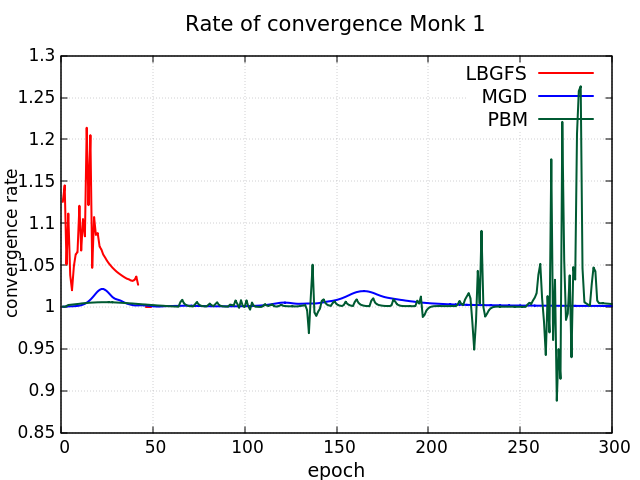
\includegraphics[width=\linewidth]{data/Comparison/Monk1/Monk1_CR_standard.png}
		\subcaption{Standard}
	\end{minipage}%
	\begin{minipage}[t]{0.5\linewidth}
		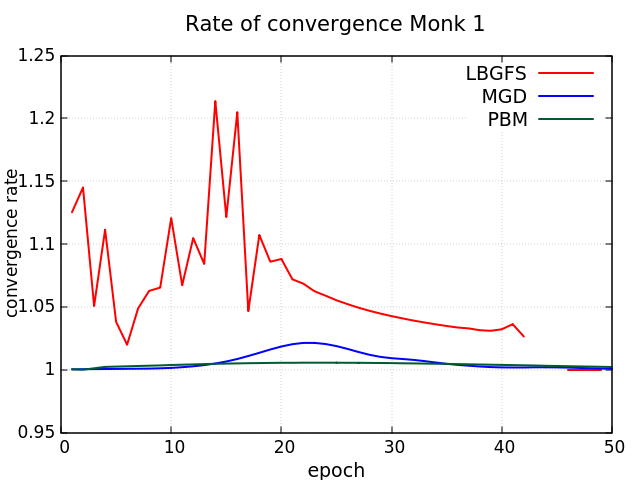
\includegraphics[width=\linewidth]{data/Comparison/Monk1/Monk1_CR_zoom.png}
		\subcaption{Zoom}
	\end{minipage}
	\caption{Converge rate comparison Monk 1 of configurations defined in table \ref{tab:nets_comp}}
	\label{CR-Monk1}
\end{figure}
\begin{figure}[H]
	\centering
	\begin{minipage}[t]{0.5\linewidth}
		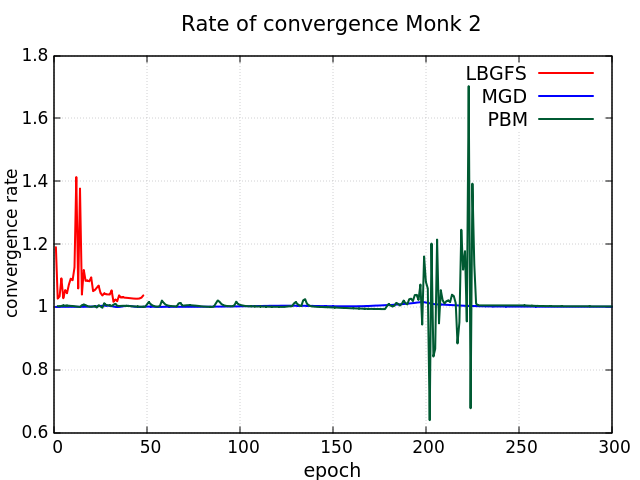
\includegraphics[width=\linewidth]{data/Comparison/Monk2/Monk2_CR_standard.png}
		\subcaption{Standard}
	\end{minipage}%
	\begin{minipage}[t]{0.5\linewidth}
		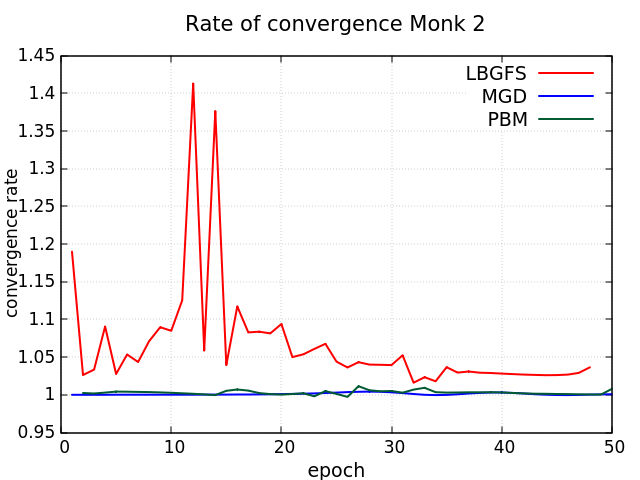
\includegraphics[width=\linewidth]{data/Comparison/Monk2/Monk2_CR_zoom.png}
		\subcaption{Zoom}
	\end{minipage}
	\caption{Converge rate comparison Monk 2 of configurations defined in table \ref{tab:nets_comp}}
	\label{CR-Monk2}
\end{figure}
\begin{figure}[H]
	\centering
	\begin{minipage}[t]{0.5\linewidth}
		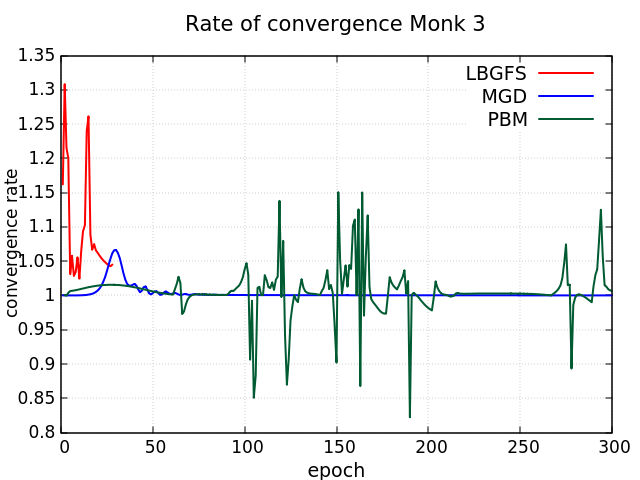
\includegraphics[width=\linewidth]{data/Comparison/Monk3/Monk3_CR_standard.png}
		\subcaption{Standard}
	\end{minipage}%
	\begin{minipage}[t]{0.5\linewidth}
		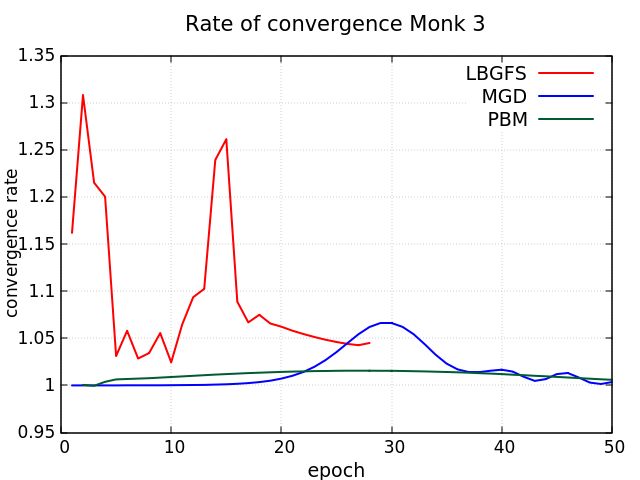
\includegraphics[width=\linewidth]{data/Comparison/Monk3/Monk3_CR_zoom.png}
		\subcaption{Zoom}
	\end{minipage}
	\caption{Converge rate comparison Monk 3 of configurations defined in table \ref{tab:nets_comp}}
	\label{CR-Monk3}
\end{figure}

\subsubsection{Computational time}
To compare the computational time behaviour of the implemented algorithm, we decided to display their curves in the plots \ref{CT-Monk1},\ref{CT-Monk2}, and \ref{CT-Monk3}. We can observe that, as expected from the theory, the most expensive method is the Proximal Bundle Method because of the time spent on the resolution of a quadratic programming problem by an external solver. As we can see in table \ref{tab:nets_res} the computational time of the Momentum Descent Approach is always lower than the others, it means that it is faster to reach a good value of the error in the Monks dataset. Moreover, we can infer that the L-BFGS algorithm gives us the best approximation of the objective function, meanwhile at a greater cost for each iteration. This is due to the better descent direction given by the approximation of the Hessian. Also, for this approximation, it has to pay some high computational costs that usually do not allow to use this kind of approach in all the situation. 

\begin{figure}[H]
	\centering
	\begin{minipage}[t]{0.5\linewidth}
		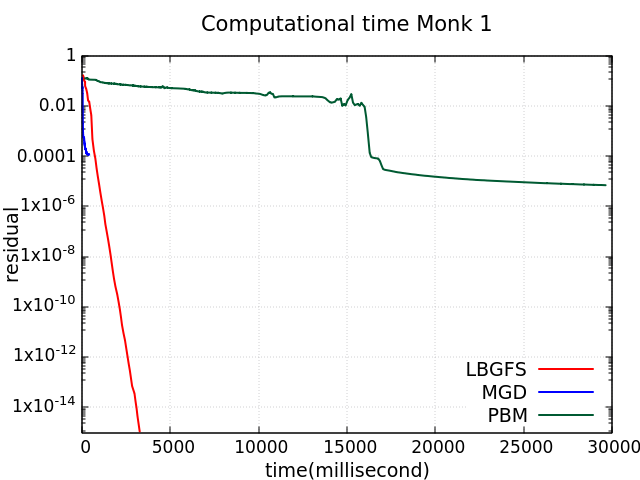
\includegraphics[width=\linewidth]{data/Comparison/Monk1/Monk1_CT_Comparison_log_standard.png}
		\subcaption{Standard}
	\end{minipage}%
	\begin{minipage}[t]{0.5\linewidth}
		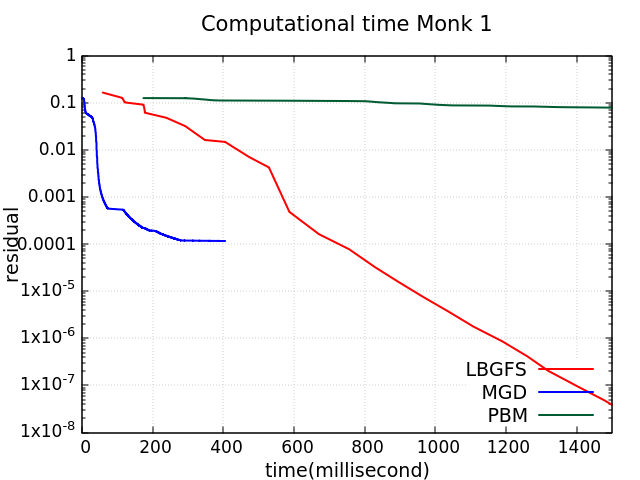
\includegraphics[width=\linewidth]{data/Comparison/Monk1/Monk1_CT_Comparison_log_zoom.png}
		\subcaption{Zoom}
	\end{minipage}
	\caption{Computational time comparison Monk 1 of configurations defined in table \ref{tab:nets_comp}}
	\label{CT-Monk1}
\end{figure}
\begin{figure}[H]
	\centering
	\begin{minipage}[t]{0.5\linewidth}
		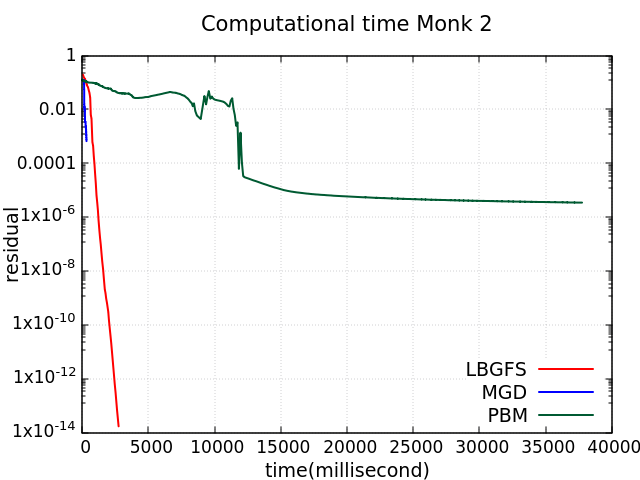
\includegraphics[width=\linewidth]{data/Comparison/Monk2/Monk2_CT_Comparison_log_standard.png}
		\subcaption{Standard}
	\end{minipage}%
	\begin{minipage}[t]{0.5\linewidth}
		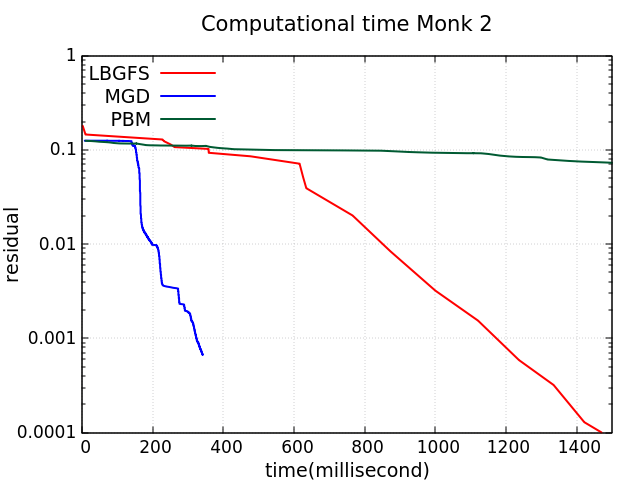
\includegraphics[width=\linewidth]{data/Comparison/Monk2/Monk2_CT_Comparison_log_zoom.png}
		\subcaption{Zoom}
	\end{minipage}
	\caption{Computational time comparison Monk 2 of configurations defined in table \ref{tab:nets_comp}}
	\label{CT-Monk2}
\end{figure}
\begin{figure}[H]
	\centering
	\begin{minipage}[t]{0.5\linewidth}
		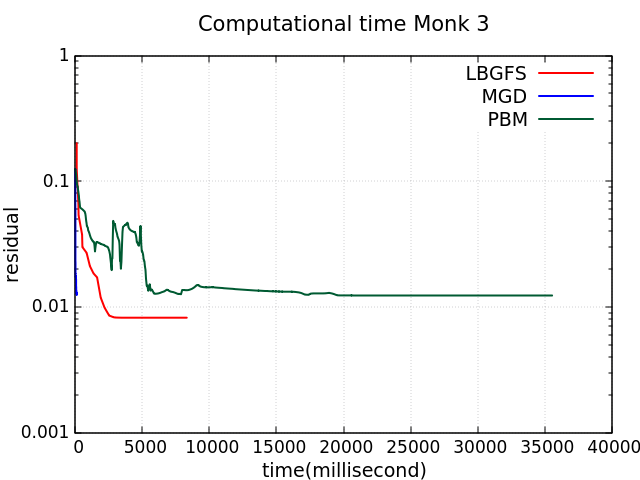
\includegraphics[width=\linewidth]{data/Comparison/Monk3/Monk3_CT_Comparison_log_standard.png}
		\subcaption{Standard}
	\end{minipage}%
	\begin{minipage}[t]{0.5\linewidth}
		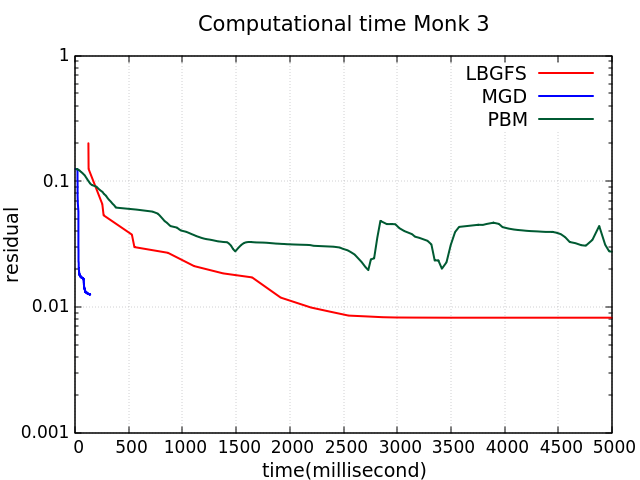
\includegraphics[width=\linewidth]{data/Comparison/Monk3/Monk3_CT_Comparison_log_zoom.png}
		\subcaption{Zoom}
	\end{minipage}
	\caption{Computational time comparison Monk 3 of configurations defined in table \ref{tab:nets_comp}}
	\label{CT-Monk3}
\end{figure}



\subsubsection{Gradient norm convergence speed}
Here we can observe that the behaviour of the algorithms follows what we stated before in the theory about their convergence speed. We view from the plots that the norm of the gradient is not smooth in all the Monks dataset. In our opinion, this is due to the starting point of the training and the non-convexity of the objective function. We know from the theory that these methods tend to have some problems with the local minimum. Also, we can observe that at a certain point the norm tends to stabilize and converge to zero. Therefore, we can infer that in the neighbourhood of the last visited minima there are no other minimum better than itself and the search of the best minima can stop.
\begin{figure}[H]
	\centering
	\begin{minipage}[t]{0.5\linewidth}
		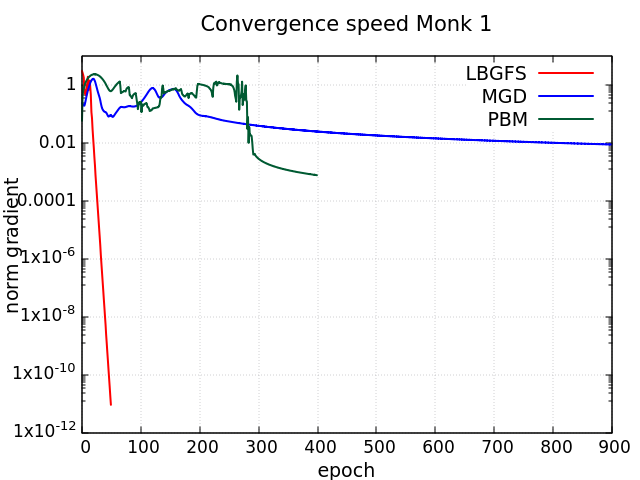
\includegraphics[width=\linewidth]{data/Comparison/Monk1/Monk1_CS_Comparison_log_standard.png}
		\subcaption{Standard}
	\end{minipage}%
	\begin{minipage}[t]{0.5\linewidth}
		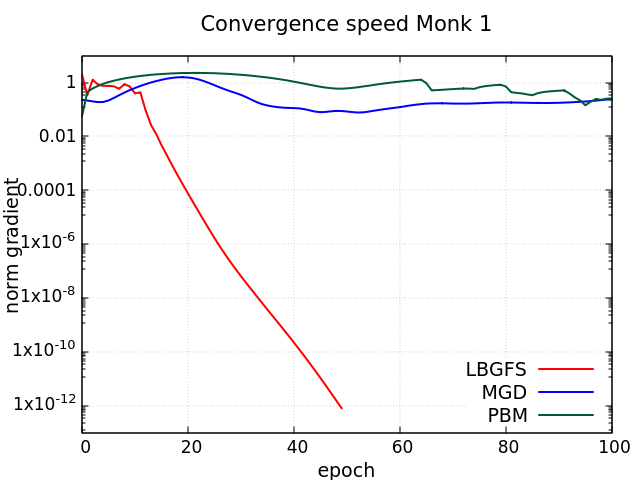
\includegraphics[width=\linewidth]{data/Comparison/Monk1/Monk1_CS_Comparison_log_zoom.png}
		\subcaption{Zoom}
	\end{minipage}
	\caption{Converge speed comparison Monk 1 of configurations defined in table \ref{tab:nets_comp}}
	\label{CS-Monk1}
\end{figure}
\begin{figure}[H]
	\centering
	\begin{minipage}[t]{0.5\linewidth}
		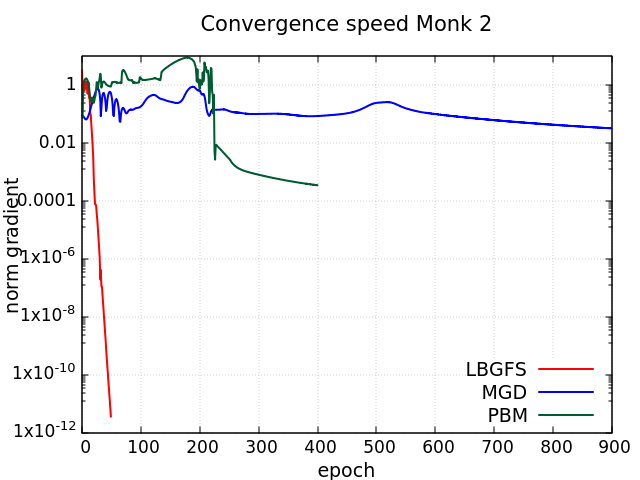
\includegraphics[width=\linewidth]{data/Comparison/Monk2/Monk2_CS_Comparison_log_standard.png}
		\subcaption{Standard}
	\end{minipage}%
	\begin{minipage}[t]{0.5\linewidth}
		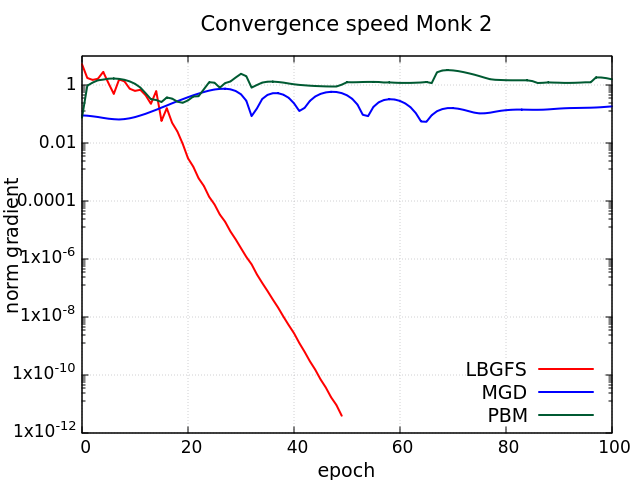
\includegraphics[width=\linewidth]{data/Comparison/Monk2/Monk2_CS_Comparison_log_zoom.png}
		\subcaption{Zoom}
	\end{minipage}
	 \caption{Converge speed comparison Monk 2 of configurations defined in table \ref{tab:nets_comp}}
	 \label{CS-Monk2}
\end{figure}
\begin{figure}[H]
	\centering
	\begin{minipage}[t]{0.5\linewidth}
		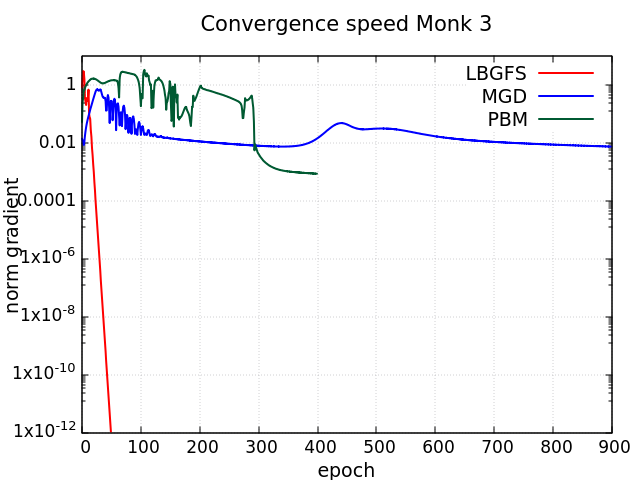
\includegraphics[width=\linewidth]{data/Comparison/Monk3/Monk3_CS_Comparison_log_standard.png}
		\subcaption{Standard}
	\end{minipage}%
	\begin{minipage}[t]{0.5\linewidth}
		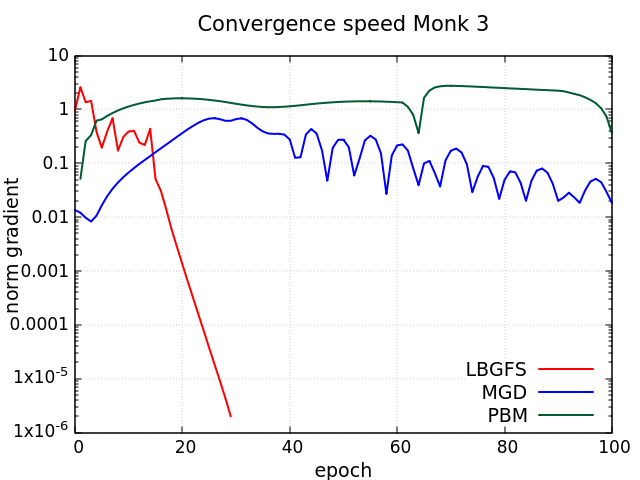
\includegraphics[width=\linewidth]{data/Comparison/Monk3/Monk3_CS_Comparison_log_zoom.png}
		\subcaption{Zoom}
	\end{minipage}
	\caption{Converge speed comparison Monk 3 of configurations defined in table \ref{tab:nets_comp}}
	\label{CS-onk3}
\end{figure}

\subsubsection{Residual}
The residual value is obtained by the following formula: $ f(x_k) - f^*$ where k is the index of the iteration. The plots of the residual value obtained from the configurations in the table \ref{tab:nets_comp} are shown below. The residual curves obtained, also with an enlargement for each of them, are shown below.

\begin{figure}[H]
	\centering
	\begin{minipage}[t]{0.5\linewidth}
		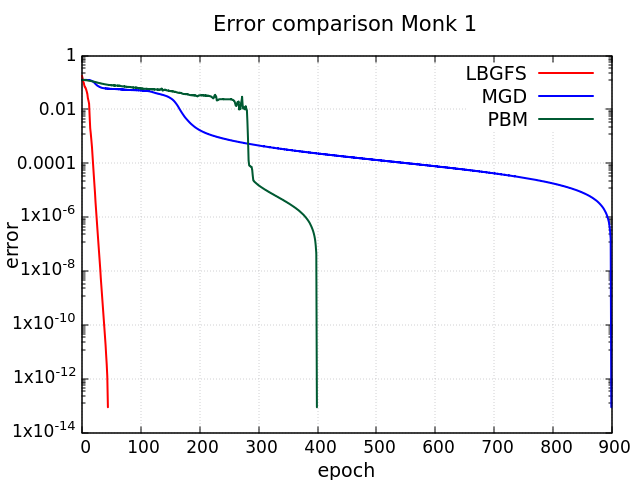
\includegraphics[width=\linewidth]{data/Comparison/Monk1/Monk1_R_Comparison_log_standard.png}
		\subcaption{Standard}
	\end{minipage}%
	\begin{minipage}[t]{0.5\linewidth}
		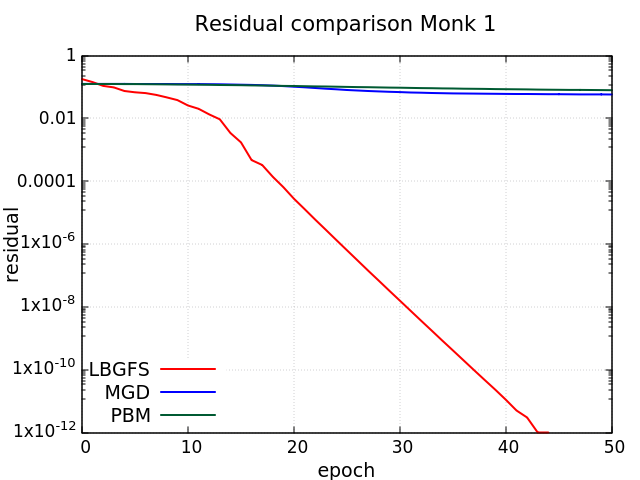
\includegraphics[width=\linewidth]{data/Comparison/Monk1/Monk1_R_Comparison_log_zoom.png}
		\subcaption{Zoom}
	\end{minipage}
	\caption{Residual comparison Monk 1 of configurations defined in table \ref{tab:nets_comp}}
	\label{R-Monk1}
\end{figure}
\begin{figure}[H]
	\centering
	\begin{minipage}[t]{0.5\linewidth}
		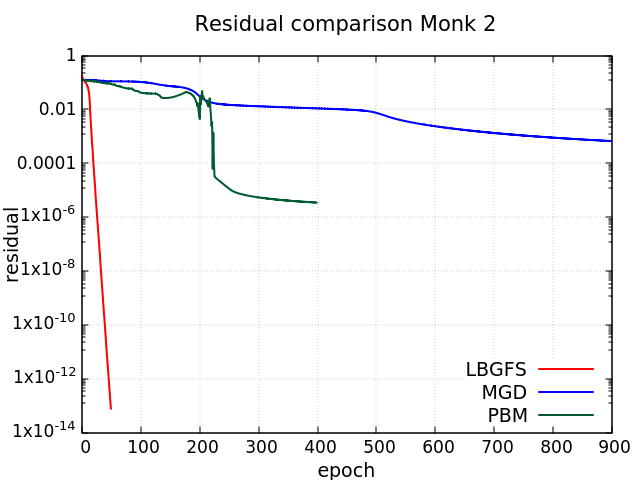
\includegraphics[width=\linewidth]{data/Comparison/Monk2/Monk2_R_Comparison_log_standard.png}
		\subcaption{Standard}
	\end{minipage}%
	\begin{minipage}[t]{0.5\linewidth}
		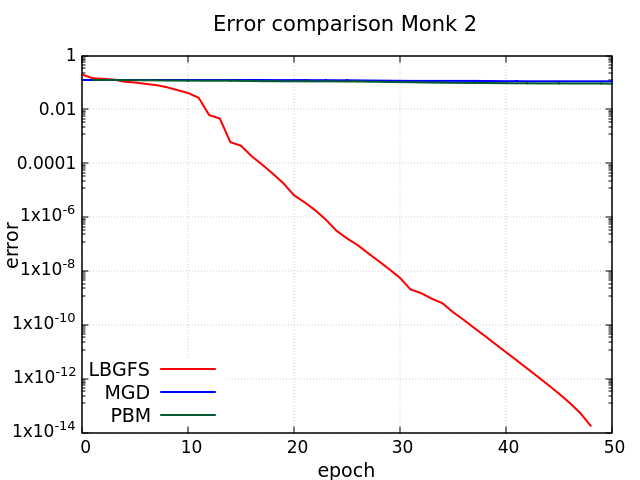
\includegraphics[width=\linewidth]{data/Comparison/Monk2/Monk2_R_Comparison_log_zoom.png}
		\subcaption{Zoom}
	\end{minipage}
	\caption{Residual comparison Monk 2 of configurations defined in table \ref{tab:nets_comp}}
	\label{R-Monk2}
\end{figure}
\begin{figure}[H]
	\centering
	\begin{minipage}[t]{0.5\linewidth}
		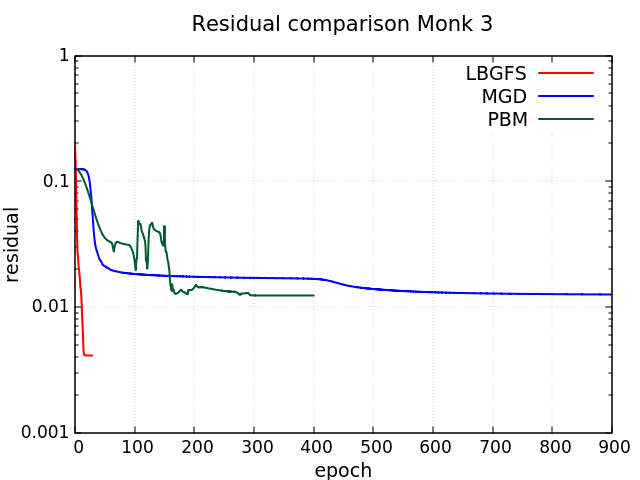
\includegraphics[width=\linewidth]{data/Comparison/Monk3/Monk3_R_Comparison_log_standard.png}
		\subcaption{Standard}
	\end{minipage}%
	\begin{minipage}[t]{0.5\linewidth}
		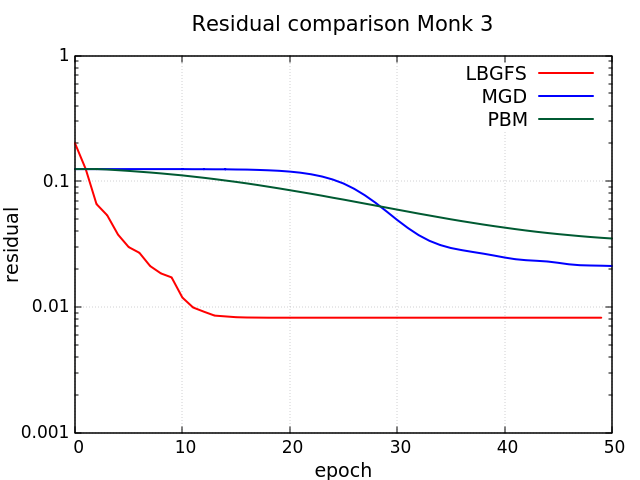
\includegraphics[width=\linewidth]{data/Comparison/Monk3/Monk3_R_Comparison_log_zoom.png}
		\subcaption{Zoom}
	\end{minipage}
	\caption{Residual comparison Monk 3 of configurations defined in table \ref{tab:nets_comp}}
	\label{R-Monk3}
\end{figure}
%\section{Code}

%Coding the algorithms is a major part of the project. Languages that are often convenient for numerical computationare (depending on the task) Matlab, Python, and C/C++, but we impose no strict requirements; you can use anyreasonable programming language.You are expected to implement the algorithm yourself; it shouldnotbe a single line of library call. However,you can use the numerical libraries of your language of choice for some of the individual steps: for instance, you canusenumpy.linalg.normto evaluate the error, or Matlab’sA \ bto solve a linear system that appears as a sub-step(unless, of course, writing a linear solver to compute that solution is a main task in your project).You can (and should) also use numerical libraries to compare their results to yours: for instance, checking if youralgorithm is faster or slower than Matlab’squadprog, if it produces (up to a tolerance) the same objective value, orhow the residual of your solution compares with that produced byA \ b.When in doubt if you should use a library, feel free to ask us.Your goal for this project is implementing and testing numerical algorithms: software engineering practices such asa full test suite, or pages of production-quality documentation, arenotrequired. That said, we appreciate well-writtenand well-documented code (who doesn’t?). You are free to use tools such asgitto ease your work, if you are familiarwith them (but giving us a pointer to thegitrepository is not the expected way to communicate with us).
\section{Conclusions}
The project made us understand how the theory seen during the course was strictly correlated with the implementation of a real neural network library. Thanks to MONK's dataset we discovered how really the regularization techniques prevent overfitting controlling model complexity. We understood the importance of choosing a good model and how to do it using grid search and k-cross validation. The hyperparameter tuning was also the most difficult phase with the debugging and testing of the backpropagation algorithm. This experience thought us the foundations of learning algorithms on neural networks on which many machine learning frameworks are based today. The experience of working in a team has allowed us to refine our knowledge about how real work experience is done and helped us not to break down during development.



\begin{thebibliography}{9}

	\bibitem{numerical} 
	Jorge Nocedal  Stephen J. Wright.
	\textit{Numerical Optimization}. Springer, (2nd Edition, 2006).

	\bibitem{PaperL-BFQS} 
	Dong C. Liu and Jorge Nocedal.
	\textit{On the limited memory BFGS method for large scale optimization}. Mathematical Programming 45 (1989), pp. 503-528.
	\\\texttt{https://people.sc.fsu.edu/~inavon/5420a/liu89limited.pdf}
		
	\bibitem{gradientProof} 
	Léon Bottou, Frank E. Curtis, and Jorge Nocedal.
	\textit{Optimization methods for largescale machine learning}. 
	[\textit{ Analyses of Stochastic Gradient Methods}]. Chapter 4.
	2016.
	
	\bibitem{armadillo} 		
	Conrad Sanderson and Ryan Curtin. 
	\textit{Armadillo: a template-based C++ library for linear algebra}. 
	\\\texttt{http://arma.sourceforge.net/armadillo\_joss\_2016.pdf}

	
	\bibitem{haykin} 
	Simon Haykin. 
	\textit{Neural Networks and Learning Machines}. 
	Prentice-Hall, (3rd Edition, 2008).


	\bibitem{mitchell} 
	T. M. Mitchell. 
	\textit{Machine learning}. 
	McGraw-Hill, 1997.
	
	\bibitem{goodfellow} 
	I. Goodfellow, Y. Bengio, A. Courville. 
	\textit{Deep Learning}. 
	MIT Press,  2016.
	
	\bibitem{monk} 
	S.B. Thrun, J. Bala, E. Boloederon and I. Bratko.
	\textit{The MONK's Problems}. 
	[\textit{A performance comparison of different learning algoritms}]. Chapter 9.
	Carnegie Mellon University CMU-CS-91-197, 1991.
	\\\texttt{https://pdfs.semanticscholar.org/94c0/418c4bd9d719e1203acfd42741ebbd343073.pdf}
	


	
\end{thebibliography}




\appendix
\addcontentsline{toc}{section}{Appendice}
\section*{Appendices}
\section{Repeatability}
Each variant of the methods was tested with specific seed and initial interval of weight in order to make the execution repeatable.

\begin{table}[H]
	\centering
	\begin{tabular}{|c|c|c|c|c|}
		\hline
		\textbf{Task} &	\textbf{Method} &\textbf{ Variant} & \textbf{Initialization} &\textbf{Seed} \\ \hline
		MONK 1        &    MDA & M  0/0.3/0.6/0.9 & 1e-2, -1e-2 & 30  \\ \hline
		MONK 2        &    MDA & M  0/0.3/0.6/0.9 & 1e-2, -1e-2 & 30  \\ \hline
		MONK 3        &    MDA & M  0/0.3/0.6/0.9 & 1e-2, -1e-2 & 30  \\ \hline			
		MONK 1        &    PBM & L1  0/3e-4/5e-4/7e-4 & 1e-2, -1e-2 & 69  \\ \hline
		MONK 2        &    PBM & L1  0/3e-4/5e-4/7e-4 & 1e-2, -1e-2 & 86  \\ \hline
		MONK 3        &    PBM & L1  0/3e-4/5e-4/7e-4 & 1e-2, -1e-2 & 13  \\ \hline			
		MONK 1        &    L-BFGS & L2  0 & 1, -1 & 22  \\ \hline
		MONK 1        &    L-BFGS & L2  3e-4 & 1, -1 & 123  \\ \hline
		MONK 1        &    L-BFGS & L2  5e-4 & 1, -1 & 59  \\ \hline
		MONK 1        &    L-BFGS & L2  7e-4 & 1, -1 & 28  \\ \hline
		MONK 2        &    L-BFGS & L2  0 & 1, -1 & 2  \\ \hline
		MONK 2        &    L-BFGS & L2  3e-4 & 1, -1 & 2  \\ \hline
		MONK 2        &    L-BFGS & L2  5e-4 & 1, -1 & 399  \\ \hline
		MONK 2        &    L-BFGS & L2  7e-4 & 1, -1 & 1154  \\ \hline
		MONK 3        &    L-BFGS & L2  0 & 1, -1 & 274  \\ \hline
		MONK 3        &    L-BFGS & L2  3e-4 & 1, -1 & 39  \\ \hline
		MONK 3        &    L-BFGS & L2  5e-4 & 1, -1 & 104  \\ \hline
		MONK 3        &    L-BFGS & L2  7e-4 & 1, -1 & 37  \\ \hline
	\end{tabular}
	\caption{MONK's problems parameter.}
	\label{tab:dati}
\end{table}
\section{Monks curves}
% Momentum 
\begin{figure}[H]
	\centering
	\begin{minipage}[t]{0.5\linewidth}
		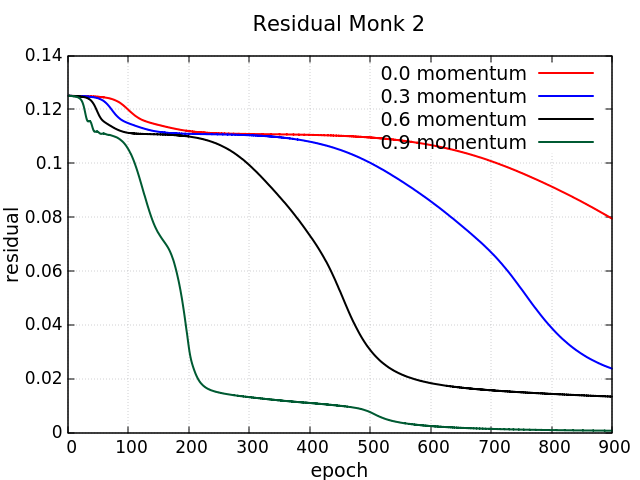
\includegraphics[width=\linewidth]{data/MGD/Monk2/M/Monk2_MGD_Residual_standard.png}
		%\subcaption{MSE}
	\end{minipage}%
	\begin{minipage}[t]{0.5\linewidth}
		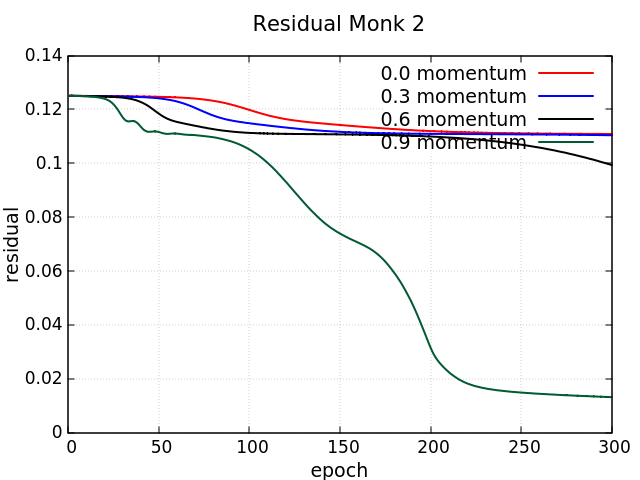
\includegraphics[width=\linewidth]{data/MGD/Monk2/M/Monk2_MGD_Residual_zoom.png}
		%\subcaption{Accuracy}
	\end{minipage}
	\caption{MDA on Monk2 dataset residual.}
\end{figure}
\begin{figure}[H]
	\centering
	\begin{minipage}[t]{0.5\linewidth}
		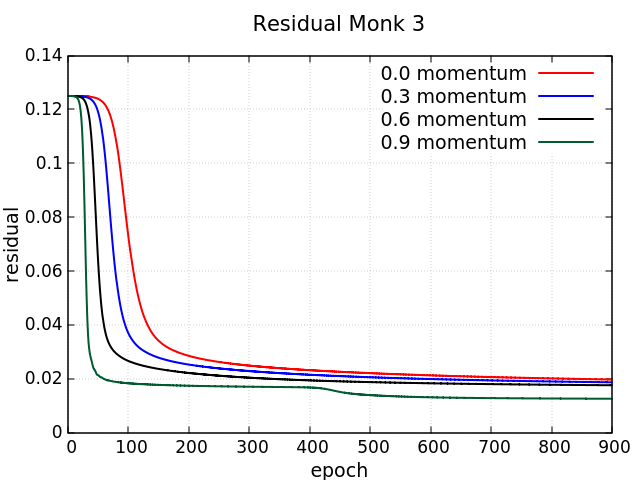
\includegraphics[width=\linewidth]{data/MGD/Monk3/M/Monk3_MGD_Residual_standard.png}
		%\subcaption{MSE}
	\end{minipage}%
	\begin{minipage}[t]{0.5\linewidth}
		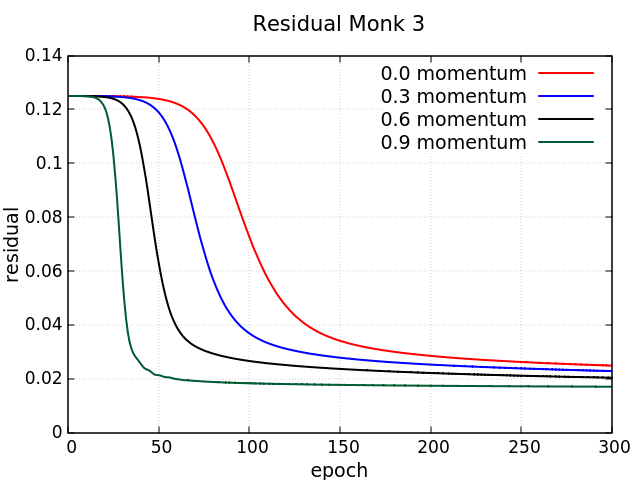
\includegraphics[width=\linewidth]{data/MGD/Monk3/M/Monk3_MGD_Residual_zoom.png}
		%\subcaption{Accuracy}
	\end{minipage}
	\caption{MDA on Monk3 dataset residual.}
\end{figure}
%Nesterov Momentum
\begin{figure}[H]
	\centering
	\begin{minipage}[t]{0.5\linewidth}
		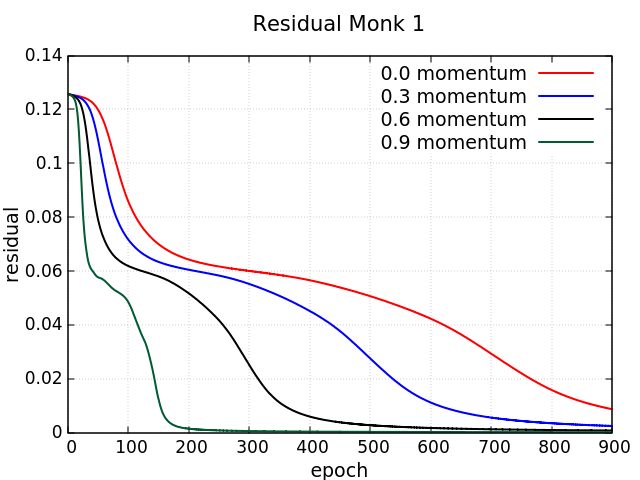
\includegraphics[width=\linewidth]{data/MGD/Monk1/NM/Monk1_NMGD_Residual_standard.png}
		%\subcaption{MSE}
	\end{minipage}%
	\begin{minipage}[t]{0.5\linewidth}
		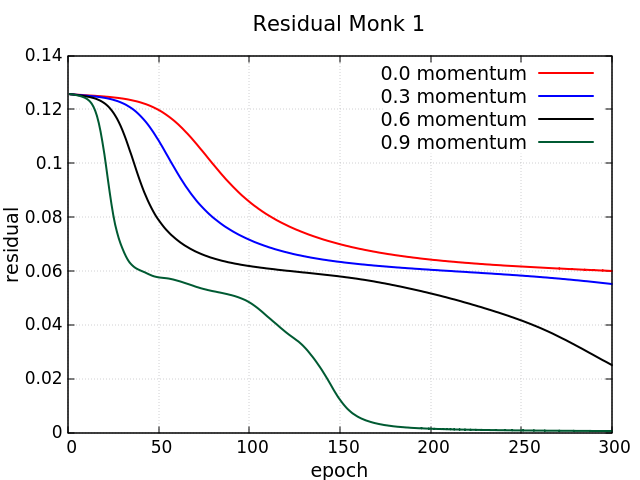
\includegraphics[width=\linewidth]{data/MGD/Monk1/NM/Monk1_NMGD_Residual_zoom.png}
		%\subcaption{Accuracy}
	\end{minipage}
	\caption{Nesterov MDA on Monk1 dataset residual.}
\end{figure}
\begin{figure}[H]
	\centering
	\begin{minipage}[t]{0.5\linewidth}
		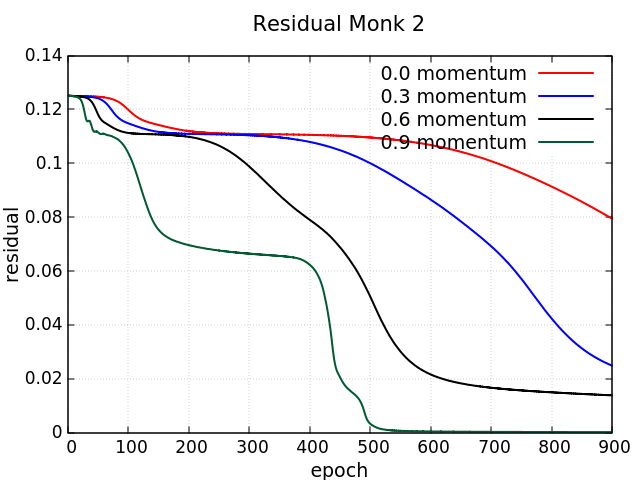
\includegraphics[width=\linewidth]{data/MGD/Monk2/NM/Monk2_NMGD_Residual_standard.png}
		%\subcaption{MSE}
	\end{minipage}%
	\begin{minipage}[t]{0.5\linewidth}
		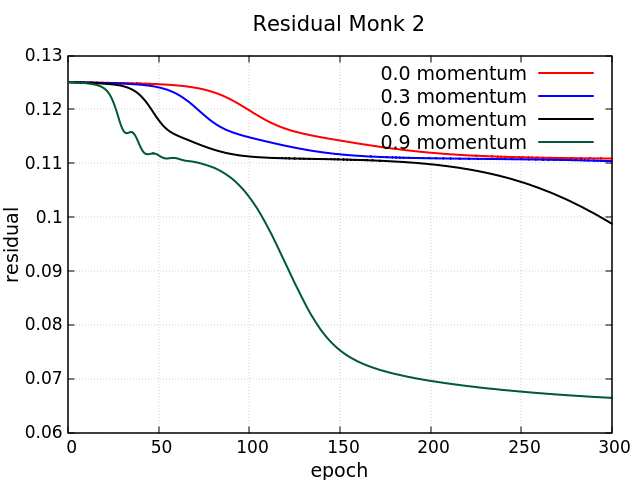
\includegraphics[width=\linewidth]{data/MGD/Monk2/NM/Monk2_NMGD_Residual_zoom.png}
		%\subcaption{Accuracy}
	\end{minipage}
	\caption{Nesterov MDA on Monk2 dataset residual.}
\end{figure}
\begin{figure}[H]
	\centering
	\begin{minipage}[t]{0.5\linewidth}
		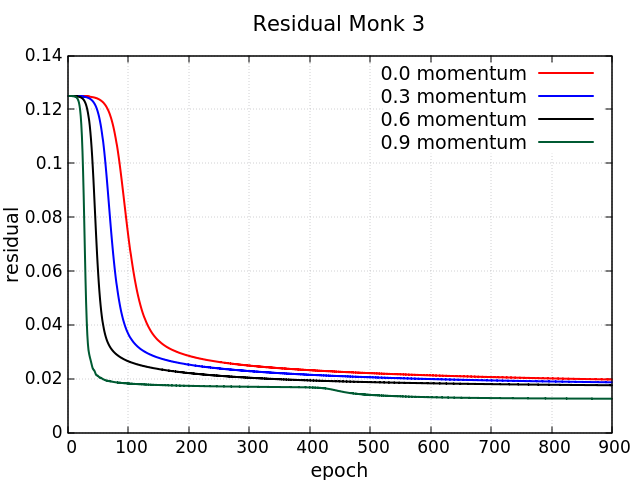
\includegraphics[width=\linewidth]{data/MGD/Monk3/NM/Monk3_NMGD_Residual_standard.png}
		%\subcaption{MSE}
	\end{minipage}%
	\begin{minipage}[t]{0.5\linewidth}
		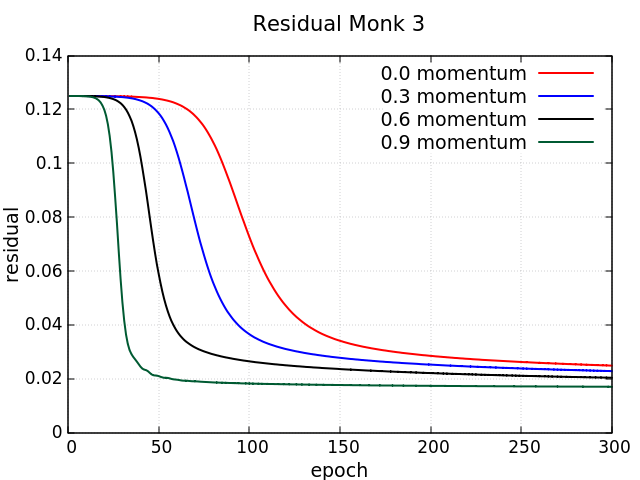
\includegraphics[width=\linewidth]{data/MGD/Monk3/NM/Monk3_NMGD_Residual_zoom.png}
		%\subcaption{Accuracy}
	\end{minipage}
	\caption{Nesterov MDA on Monk3 dataset residual.}
\end{figure}
% Bundle
\begin{figure}[H]
	\centering
	\begin{minipage}[t]{0.5\linewidth}
		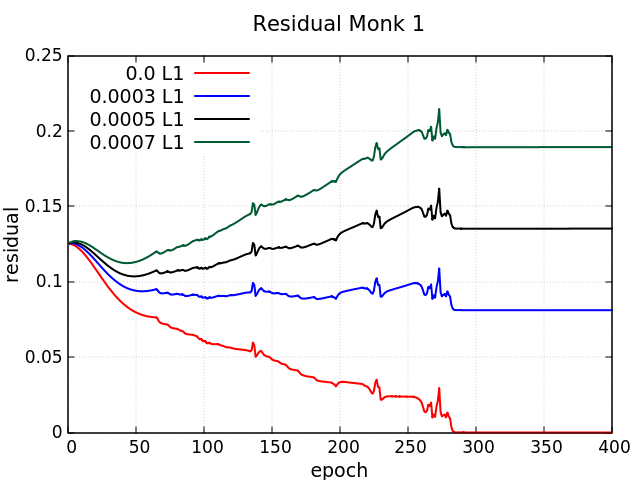
\includegraphics[width=\linewidth]{data/PBM/Monk1/Monk1_PBM_Residual_standard.png}
		%\subcaption{MSE}
	\end{minipage}%
	\begin{minipage}[t]{0.5\linewidth}
		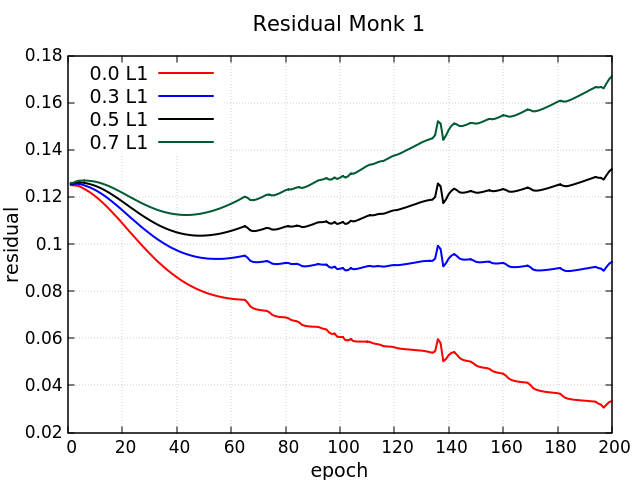
\includegraphics[width=\linewidth]{data/PBM/Monk1/Monk1_PBM_Residual_zoom.png}
		%\subcaption{Accuracy}
	\end{minipage}
	\caption{PBM on Monk1 dataset residual.}
\end{figure}
\begin{figure}[H]
	\centering
	\begin{minipage}[t]{0.5\linewidth}
		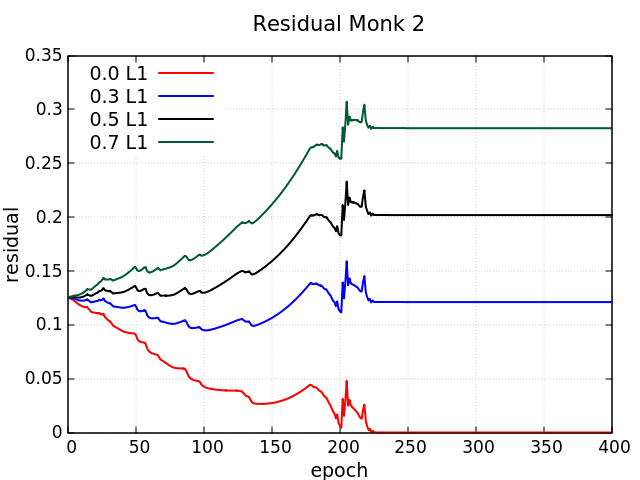
\includegraphics[width=\linewidth]{data/PBM/Monk2/Monk2_PBM_Residual_standard.png}
		%\subcaption{MSE}
	\end{minipage}%
	\begin{minipage}[t]{0.5\linewidth}
		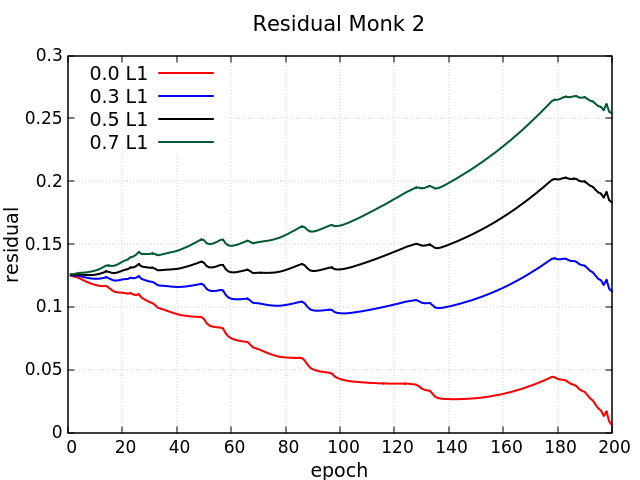
\includegraphics[width=\linewidth]{data/PBM/Monk2/Monk2_PBM_Residual_zoom.png}
		%\subcaption{Accuracy}
	\end{minipage}
	\caption{PBM on Monk2 dataset residual.}
\end{figure}
\begin{figure}[H]
	\centering
	\begin{minipage}[t]{0.5\linewidth}
		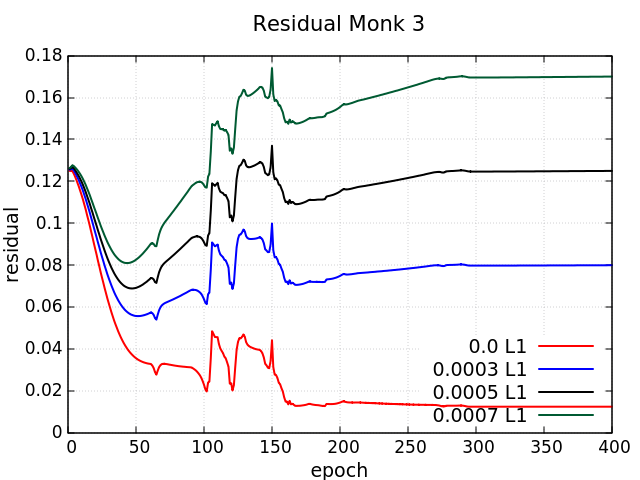
\includegraphics[width=\linewidth]{data/PBM/Monk3/Monk3_PBM_Residual_standard.png}
		%\subcaption{MSE}
	\end{minipage}%
	\begin{minipage}[t]{0.5\linewidth}
		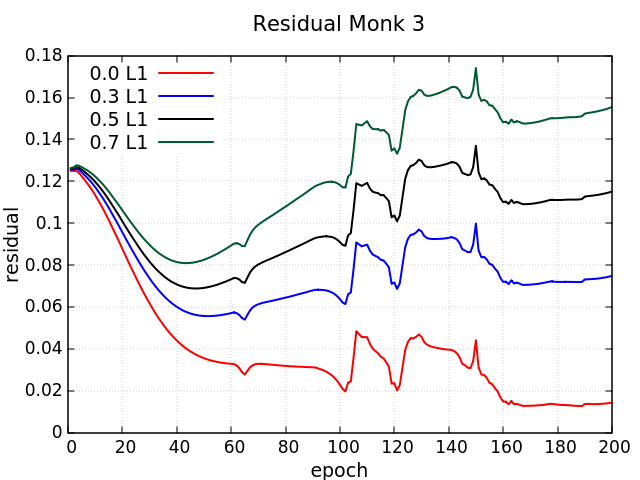
\includegraphics[width=\linewidth]{data/PBM/Monk3/Monk3_PBM_Residual_zoom.png}
		%\subcaption{Accuracy}
	\end{minipage}
	\caption{PBM on Monk3 dataset residual.}
\end{figure}
%L-BFGS
\begin{figure}[H]
	\centering
	\begin{minipage}[t]{0.5\linewidth}
		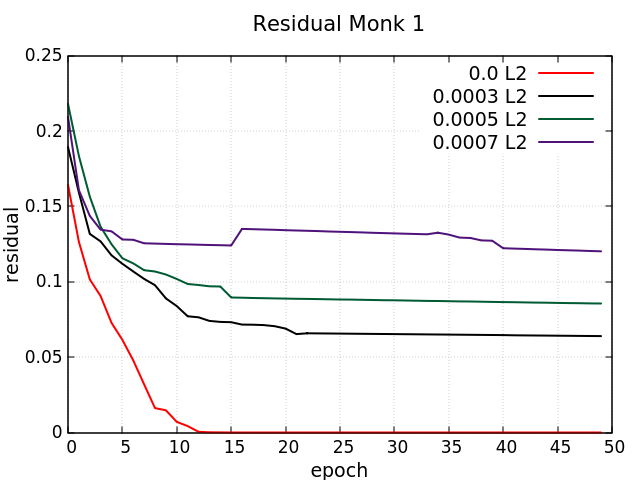
\includegraphics[width=\linewidth]{data/LBFGS/Monk1/Monk1_LBFGS_Residual_standard.png}
		%\subcaption{MSE}
	\end{minipage}%
	\begin{minipage}[t]{0.5\linewidth}
		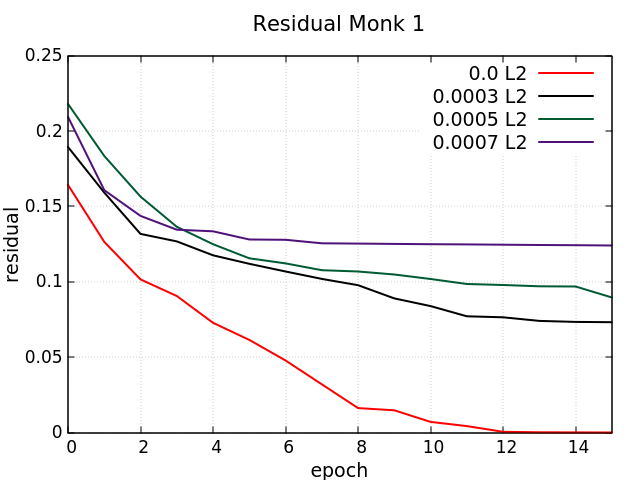
\includegraphics[width=\linewidth]{data/LBFGS/Monk1/Monk1_LBFGS_Residual_zoom.png}
		%\subcaption{Accuracy}
	\end{minipage}
	\caption{L-BFGS on Monk1 dataset residual.}
\end{figure}
\begin{figure}[H]
	\centering
	\begin{minipage}[t]{0.5\linewidth}
		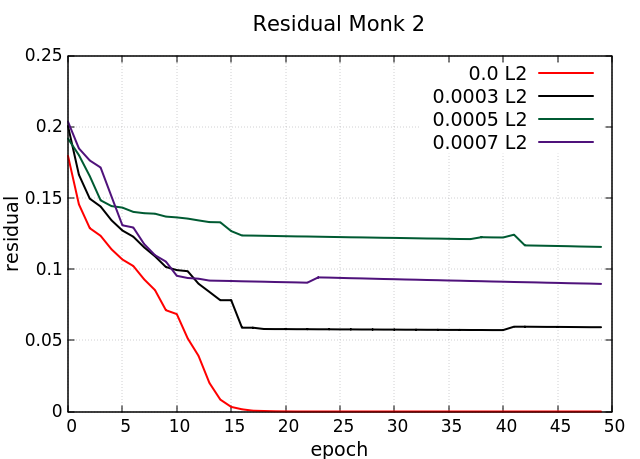
\includegraphics[width=\linewidth]{data/LBFGS/Monk2/Monk2_LBFGS_Residual_standard.png}
		%\subcaption{MSE}
	\end{minipage}%
	\begin{minipage}[t]{0.5\linewidth}
		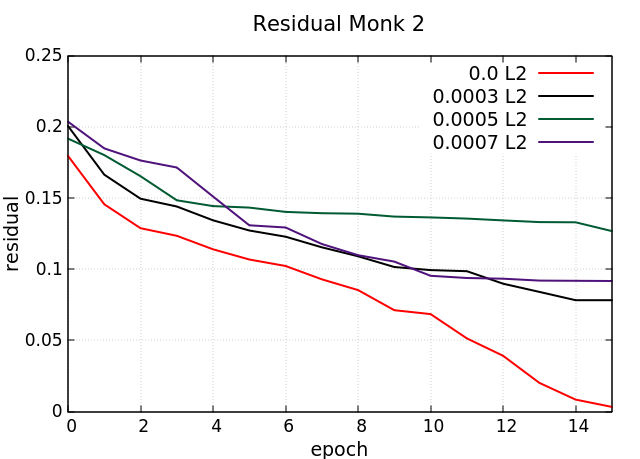
\includegraphics[width=\linewidth]{data/LBFGS/Monk2/Monk2_LBFGS_Residual_zoom.png}
		%\subcaption{Accuracy}
	\end{minipage}
	\caption{L-BFGS on Monk2 dataset residual.}
\end{figure}
\begin{figure}[H]
	\centering
	\begin{minipage}[t]{0.5\linewidth}
		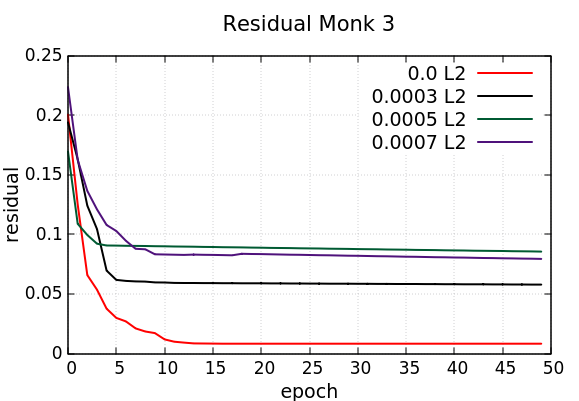
\includegraphics[width=\linewidth]{data/LBFGS/Monk3/Monk3_LBFGS_Residual_standard.png}
		%\subcaption{MSE}
	\end{minipage}%
	\begin{minipage}[t]{0.5\linewidth}
		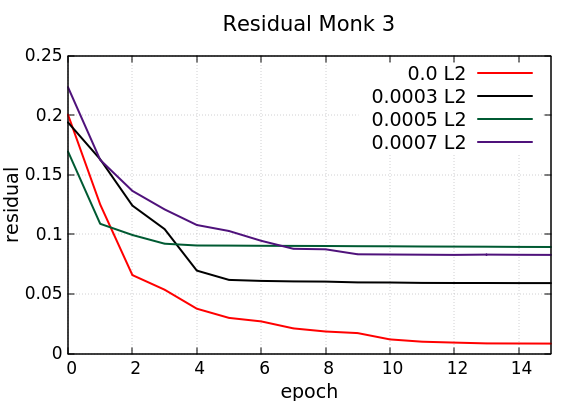
\includegraphics[width=\linewidth]{data/LBFGS/Monk3/Monk3_LBFGS_Residual_zoom.png}
		%\subcaption{Accuracy}
	\end{minipage}
	\caption{L-BFGS on Monk3 dataset residual.}
\end{figure}
\subsubsection{Computational time} 
\begin{figure}[H]
	\centering
	\begin{minipage}[t]{0.5\linewidth}
		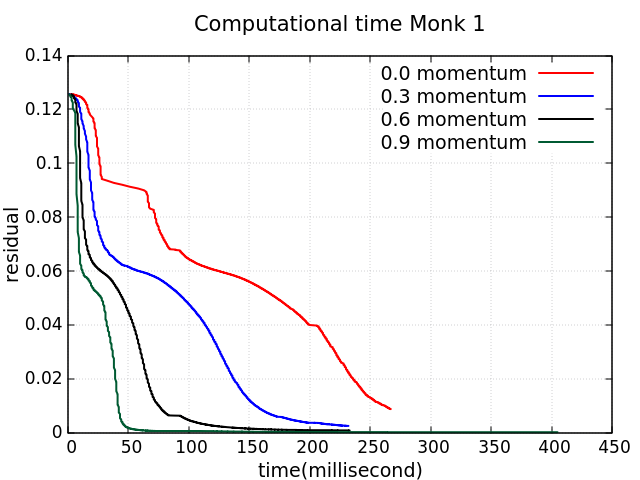
\includegraphics[width=\linewidth]{data/MGD/Monk1/M/Monk1_MGD_CT_standard.png}
		%\subcaption{MSE}
	\end{minipage}%
	\begin{minipage}[t]{0.5\linewidth}
		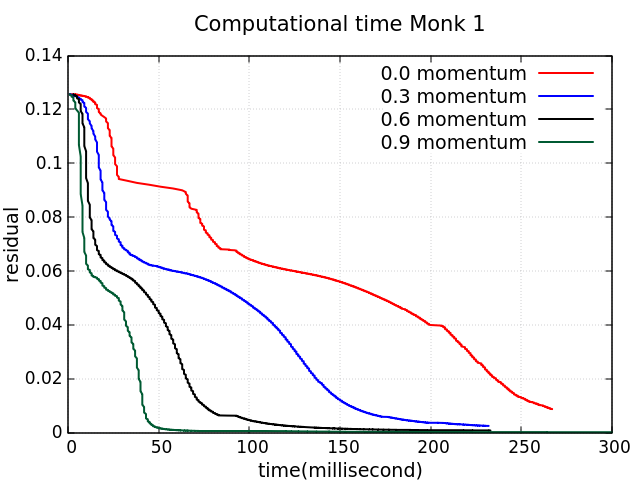
\includegraphics[width=\linewidth]{data/MGD/Monk1/M/Monk1_MGD_CT_zoom.png}
		%\subcaption{Accuracy}
	\end{minipage}
	\caption{MDA on Monk1 dataset computational time.}
\end{figure}
\begin{figure}[H]
	\centering
	\begin{minipage}[t]{0.5\linewidth}
		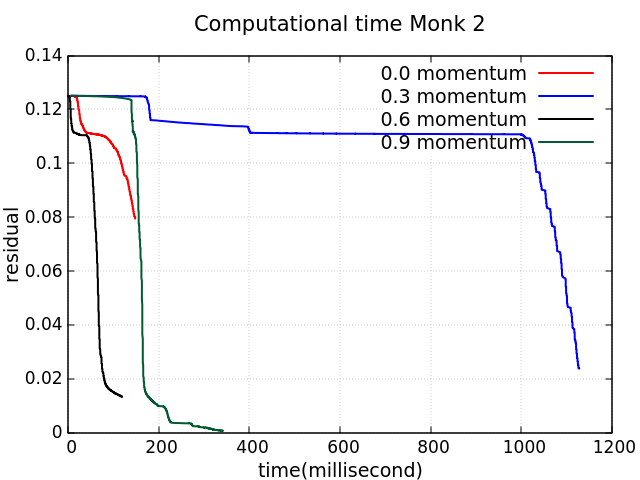
\includegraphics[width=\linewidth]{data/MGD/Monk2/M/Monk2_MGD_CT_standard.png}
		%\subcaption{MSE}
	\end{minipage}%
	\begin{minipage}[t]{0.5\linewidth}
		\includegraphics[width=\linewidth]{data/MGD/Monk2/M/Monk2_MGD_CT_zoom.png}
		%\subcaption{Accuracy}
	\end{minipage}
	\caption{MDA on Monk2 dataset computational time.}
\end{figure}
\begin{figure}[H]
	\centering
	\begin{minipage}[t]{0.5\linewidth}
		\includegraphics[width=\linewidth]{data/MGD/Monk3/M/Monk3_MGD_CT_standard.png}
		%\subcaption{MSE}
	\end{minipage}%
	\begin{minipage}[t]{0.5\linewidth}
		\includegraphics[width=\linewidth]{data/MGD/Monk3/M/Monk3_MGD_CT_zoom.png}
		%\subcaption{Accuracy}
	\end{minipage}
	\caption{MDA on Monk3 dataset computational time.}
\end{figure}
%Nesterov Momentum
\begin{figure}[H]
	\centering
	\begin{minipage}[t]{0.5\linewidth}
		\includegraphics[width=\linewidth]{data/MGD/Monk1/NM/Monk1_NMGD_CT_standard.png}
		%\subcaption{MSE}
	\end{minipage}%
	\begin{minipage}[t]{0.5\linewidth}
		\includegraphics[width=\linewidth]{data/MGD/Monk1/NM/Monk1_NMGD_CT_zoom.png}
		%\subcaption{Accuracy}
	\end{minipage}
	\caption{Nesterov MDA on Monk1 dataset computational time.}
\end{figure}
\begin{figure}[H]
	\centering
	\begin{minipage}[t]{0.5\linewidth}
		\includegraphics[width=\linewidth]{data/MGD/Monk2/NM/Monk2_NMGD_CT_standard.png}
		%\subcaption{MSE}
	\end{minipage}%
	\begin{minipage}[t]{0.5\linewidth}
		\includegraphics[width=\linewidth]{data/MGD/Monk2/NM/Monk2_NMGD_CT_zoom.png}
		%\subcaption{Accuracy}
	\end{minipage}
	\caption{Nesterov MDA on Monk2 dataset computational time.}
\end{figure}
\begin{figure}[H]
	\centering
	\begin{minipage}[t]{0.5\linewidth}
		\includegraphics[width=\linewidth]{data/MGD/Monk3/NM/Monk3_NMGD_CT_standard.png}
		%\subcaption{MSE}
	\end{minipage}%
	\begin{minipage}[t]{0.5\linewidth}
		\includegraphics[width=\linewidth]{data/MGD/Monk3/NM/Monk3_NMGD_CT_zoom.png}
		%\subcaption{Accuracy}
	\end{minipage}
	\caption{Nesterov MDA on Monk3 dataset computational time.}
\end{figure}
% Bundle
\begin{figure}[H]
	\centering
	\begin{minipage}[t]{0.5\linewidth}
		\includegraphics[width=\linewidth]{data/PBM/Monk1/Monk1_PBM_CT_standard.png}
		%\subcaption{MSE}
	\end{minipage}%
	\begin{minipage}[t]{0.5\linewidth}
		\includegraphics[width=\linewidth]{data/PBM/Monk1/Monk1_PBM_CT_zoom.png}
		%\subcaption{Accuracy}
	\end{minipage}
	\caption{PBM on Monk1 dataset computational time.}
\end{figure}
\begin{figure}[H]
	\centering
	\begin{minipage}[t]{0.5\linewidth}
		\includegraphics[width=\linewidth]{data/PBM/Monk2/Monk2_PBM_CT_standard.png}
		%\subcaption{MSE}
	\end{minipage}%
	\begin{minipage}[t]{0.5\linewidth}
		\includegraphics[width=\linewidth]{data/PBM/Monk2/Monk2_PBM_CT_zoom.png}
		%\subcaption{Accuracy}
	\end{minipage}
	\caption{PBM on Monk2 dataset computational time.}
\end{figure}
\begin{figure}[H]
	\centering
	\begin{minipage}[t]{0.5\linewidth}
		\includegraphics[width=\linewidth]{data/PBM/Monk3/Monk3_PBM_CT_standard.png}
		%\subcaption{MSE}
	\end{minipage}%
	\begin{minipage}[t]{0.5\linewidth}
		\includegraphics[width=\linewidth]{data/PBM/Monk3/Monk3_PBM_CT_zoom.png}
		%\subcaption{Accuracy}
	\end{minipage}
	\caption{PBM on Monk3 dataset computational time.}
\end{figure}
%L-BFGS
\begin{figure}[H]
	\centering
	\begin{minipage}[t]{0.5\linewidth}
		\includegraphics[width=\linewidth]{data/LBFGS/Monk1/Monk1_LBFGS_CT_standard.png}
		%\subcaption{MSE}
	\end{minipage}%
	\begin{minipage}[t]{0.5\linewidth}
		\includegraphics[width=\linewidth]{data/LBFGS/Monk1/Monk1_LBFGS_CT_zoom.png}
		%\subcaption{Accuracy}
	\end{minipage}
	\caption{L-BFGS on Monk1 dataset computational time.}
\end{figure}
\begin{figure}[H]
	\centering
	\begin{minipage}[t]{0.5\linewidth}
		\includegraphics[width=\linewidth]{data/LBFGS/Monk2/Monk2_LBFGS_CT_standard.png}
		%\subcaption{MSE}
	\end{minipage}%
	\begin{minipage}[t]{0.5\linewidth}
		\includegraphics[width=\linewidth]{data/LBFGS/Monk2/Monk2_LBFGS_CT_zoom.png}
		%\subcaption{Accuracy}
	\end{minipage}
	\caption{L-BFGS on Monk2 dataset computational time.}
\end{figure}
\begin{figure}[H]
	\centering
	\begin{minipage}[t]{0.5\linewidth}
		\includegraphics[width=\linewidth]{data/LBFGS/Monk3/Monk3_LBFGS_CT_standard.png}
		%\subcaption{MSE}
	\end{minipage}%
	\begin{minipage}[t]{0.5\linewidth}
		\includegraphics[width=\linewidth]{data/LBFGS/Monk3/Monk3_LBFGS_CT_zoom.png}
		%\subcaption{Accuracy}
	\end{minipage}
	\caption{L-BFGS on Monk3 dataset computational time.}
\end{figure}

\begin{figure}[H]
	\centering
	\begin{minipage}[t]{0.5\linewidth}
		\includegraphics[width=\linewidth]{img/Monk1_LBFGS_NoReg_standard.png}
		%\subcaption{MSE}
	\end{minipage}%
	\begin{minipage}[t]{0.5\linewidth}
		\includegraphics[width=\linewidth]{img/Monk1_LBFGS_NoReg_zoom.png}
		%\subcaption{Accuracy}
	\end{minipage}
	\caption{LBFGS convergence for MONK’s 1.}
	\label{L-BFGS-Curvature}
\end{figure}
\begin{figure}[H]
	\centering
	\begin{minipage}[t]{0.5\linewidth}
		\includegraphics[width=\linewidth]{data/MGD/Monk1/M/Monk1_MGD_CS_standard.png}
		%\subcaption{MSE}
	\end{minipage}%
	\begin{minipage}[t]{0.5\linewidth}
		\includegraphics[width=\linewidth]{data/MGD/Monk1/M/Monk1_MGD_CS_zoom.png}
		%\subcaption{Accuracy}
	\end{minipage}
	\caption{MDA on Monk1 dataset convergence speed.}
\end{figure}
\begin{figure}[H]
	\centering
	\begin{minipage}[t]{0.5\linewidth}
		\includegraphics[width=\linewidth]{data/MGD/Monk2/M/Monk2_MGD_CS_standard.png}
		%\subcaption{MSE}
	\end{minipage}%
	\begin{minipage}[t]{0.5\linewidth}
		\includegraphics[width=\linewidth]{data/MGD/Monk2/M/Monk2_MGD_CS_zoom.png}
		%\subcaption{Accuracy}
	\end{minipage}
	\caption{MDA on Monk2 dataset convergence speed.}
\end{figure}
\begin{figure}[H]
	\centering
	\begin{minipage}[t]{0.5\linewidth}
		\includegraphics[width=\linewidth]{data/MGD/Monk3/M/Monk3_MGD_CS_standard.png}
		%\subcaption{MSE}
	\end{minipage}%
	\begin{minipage}[t]{0.5\linewidth}
		\includegraphics[width=\linewidth]{data/MGD/Monk3/M/Monk3_MGD_CS_zoom.png}
		%\subcaption{Accuracy}
	\end{minipage}
	\caption{MDA on Monk3 dataset convergence speed.}
\end{figure}
%Nesterov Momentum
\begin{figure}[H]
	\centering
	\begin{minipage}[t]{0.5\linewidth}
		\includegraphics[width=\linewidth]{data/MGD/Monk1/NM/Monk1_NMGD_CS_standard.png}
		%\subcaption{MSE}
	\end{minipage}%
	\begin{minipage}[t]{0.5\linewidth}
		\includegraphics[width=\linewidth]{data/MGD/Monk1/NM/Monk1_NMGD_CS_zoom.png}
		%\subcaption{Accuracy}
	\end{minipage}
	\caption{Nesterov MDA on Monk1 dataset convergence speed.}
\end{figure}
\begin{figure}[H]
	\centering
	\begin{minipage}[t]{0.5\linewidth}
		\includegraphics[width=\linewidth]{data/MGD/Monk2/NM/Monk2_NMGD_CS_standard.png}
		%\subcaption{MSE}
	\end{minipage}%
	\begin{minipage}[t]{0.5\linewidth}
		\includegraphics[width=\linewidth]{data/MGD/Monk2/NM/Monk2_NMGD_CS_zoom.png}
		%\subcaption{Accuracy}
	\end{minipage}
	\caption{Nesterov MDA on Monk2 dataset convergence speed.}
\end{figure}
\begin{figure}[H]
	\centering
	\begin{minipage}[t]{0.5\linewidth}
		\includegraphics[width=\linewidth]{data/MGD/Monk3/NM/Monk3_NMGD_CS_standard.png}
		%\subcaption{MSE}
	\end{minipage}%
	\begin{minipage}[t]{0.5\linewidth}
		\includegraphics[width=\linewidth]{data/MGD/Monk3/NM/Monk3_NMGD_CS_zoom.png}
		%\subcaption{Accuracy}
	\end{minipage}
	\caption{Nesterov MDA on Monk3 dataset convergence speed.}
\end{figure}
% Bundle
\begin{figure}[H]
	\centering
	\begin{minipage}[t]{0.5\linewidth}
		\includegraphics[width=\linewidth]{data/PBM/Monk1/Monk1_PBM_CS_standard.png}
		%\subcaption{MSE}
	\end{minipage}%
	\begin{minipage}[t]{0.5\linewidth}
		\includegraphics[width=\linewidth]{data/PBM/Monk1/Monk1_PBM_CS_zoom.png}
		%\subcaption{Accuracy}
	\end{minipage}
	\caption{PBM on Monk1 dataset convergence speed.}
\end{figure}
\begin{figure}[H]
	\centering
	\begin{minipage}[t]{0.5\linewidth}
		\includegraphics[width=\linewidth]{data/PBM/Monk2/Monk2_PBM_CS_standard.png}
		%\subcaption{MSE}
	\end{minipage}%
	\begin{minipage}[t]{0.5\linewidth}
		\includegraphics[width=\linewidth]{data/PBM/Monk2/Monk2_PBM_CS_zoom.png}
		%\subcaption{Accuracy}
	\end{minipage}
	\caption{PBM on Monk2 dataset convergence speed.}
\end{figure}
\begin{figure}[H]
	\centering
	\begin{minipage}[t]{0.5\linewidth}
		\includegraphics[width=\linewidth]{data/PBM/Monk3/Monk3_PBM_CS_standard.png}
		%\subcaption{MSE}
	\end{minipage}%
	\begin{minipage}[t]{0.5\linewidth}
		\includegraphics[width=\linewidth]{data/PBM/Monk3/Monk3_PBM_CS_zoom.png}
		%\subcaption{Accuracy}
	\end{minipage}
	\caption{PBM on Monk3 dataset convergence speed.}
\end{figure}
%L-BFGS
\begin{figure}[H]
	\centering
	\begin{minipage}[t]{0.5\linewidth}
		\includegraphics[width=\linewidth]{data/LBFGS/Monk1/Monk1_LBFGS_CS_standard.png}
		%\subcaption{MSE}
	\end{minipage}%
	\begin{minipage}[t]{0.5\linewidth}
		\includegraphics[width=\linewidth]{data/LBFGS/Monk1/Monk1_LBFGS_CS_zoom.png}
		%\subcaption{Accuracy}
	\end{minipage}
	\caption{L-BFGS on Monk1 dataset convergence speed.}
\end{figure}
\begin{figure}[H]
	\centering
	\begin{minipage}[t]{0.5\linewidth}
		\includegraphics[width=\linewidth]{data/LBFGS/Monk2/Monk2_LBFGS_CS_standard.png}
		%\subcaption{MSE}
	\end{minipage}%
	\begin{minipage}[t]{0.5\linewidth}
		\includegraphics[width=\linewidth]{data/LBFGS/Monk2/Monk2_LBFGS_CS_zoom.png}
		%\subcaption{Accuracy}
	\end{minipage}
	\caption{L-BFGS on Monk2 dataset convergence speed.}
\end{figure}
\begin{figure}[H]
	\centering
	\begin{minipage}[t]{0.5\linewidth}
		\includegraphics[width=\linewidth]{data/LBFGS/Monk3/Monk3_LBFGS_CS_standard.png}
		%\subcaption{MSE}
	\end{minipage}%
	\begin{minipage}[t]{0.5\linewidth}
		\includegraphics[width=\linewidth]{data/LBFGS/Monk3/Monk3_LBFGS_CS_zoom.png}
		%\subcaption{Accuracy}
	\end{minipage}
	\caption{L-BFGS on Monk3 dataset convergence speed.}
\end{figure}
\subsubsection{Residual}
\begin{figure}[H]
	\centering
	\begin{minipage}[t]{0.5\linewidth}
		\includegraphics[width=\linewidth]{data/MGD/Monk1/M/Monk1_MGD_Residual_standard.png}
		%\subcaption{MSE}
	\end{minipage}%
	\begin{minipage}[t]{0.5\linewidth}
		\includegraphics[width=\linewidth]{data/MGD/Monk1/M/Monk1_MGD_Residual_zoom.png}
		%\subcaption{Accuracy}
	\end{minipage}
	\caption{MDA on Monk1 dataset residual.}
\end{figure}


\newpage
\begin{thebibliography}{9}

	\bibitem{numerical} 
	Jorge Nocedal  Stephen J. Wright.
	\textit{Numerical Optimization}. Springer, (2nd Edition, 2006).

	\bibitem{PaperL-BFQS} 
	Dong C. Liu and Jorge Nocedal.
	\textit{On the limited memory BFGS method for large scale optimization}. Mathematical Programming 45 (1989), pp. 503-528.
	\\\texttt{https://people.sc.fsu.edu/\textasciitilde inavon/5420a/liu89limited.pdf}
	
	\bibitem{backpropagation} 		
	David E. Rumelhart, Geoffrey E. Hinton \& Ronald J. Williams . 
	\textit{Learning representation by back-propagating errors}. 
	\\\texttt{https://www.nature.com/articles/323533a0}
	
		
	\bibitem{gradientProof} 
	Léon Bottou, Frank E. Curtis, and Jorge Nocedal.
	\textit{Optimization methods for largescale machine learning}. 
	[\textit{ Analyses of Stochastic Gradient Methods}]. Chapter 4.
	2016.
	
	\bibitem{armadillo} 		
	Conrad Sanderson and Ryan Curtin. 
	\textit{Armadillo: a template-based C++ library for linear algebra}. 
	\\\texttt{http://arma.sourceforge.net/armadillo\_joss\_2016.pdf}

	
	\bibitem{haykin} 
	Simon Haykin. 
	\textit{Neural Networks and Learning Machines}. 
	Prentice-Hall, (3rd Edition, 2008).


	\bibitem{mitchell} 
	T. M. Mitchell. 
	\textit{Machine learning}. 
	McGraw-Hill, 1997.
	
	\bibitem{goodfellow} 
	I. Goodfellow, Y. Bengio, A. Courville. 
	\textit{Deep Learning}. 
	MIT Press,  2016.
	
	\bibitem{bert03} 
	D.P. Bertsekas.
	\textit{Nonlinear Programming}. 
	Second edition. Athena Scientific, 2003.
	
	\bibitem{PaperBM} 
	A. Frangioni.
	\textit{Standard Bundle Methods: Untrusted Models and Duality}.
	\\\texttt{http://pages.di.unipi.it/frangio/abstracts.html\#NDOB18}
	
	\bibitem{PBM} 
	Marko M. M\"akel\"a, Napsu Karmitsa and Outi Wilppu.
	\textit{Proximal Bundle Method for Nonsmooth andNonconvex Multiobjective Optimization}.
	\\\texttt{http://napsu.karmitsa.fi/publications/pbm.pdf}
	
	\bibitem{NonOpt} 
	Andrzej Ruszczyński.
	\textit{Nonlinear Optimization}. Princeton University Press. 
	
	\bibitem{CBM} 
	Y. Du and A. Ruszczyński.
	\textit{Rate of Convergence of the Bundle Method}. Journal  of  Optimization Theory and Applications.
	\\\texttt{https://arxiv.org/pdf/1609.00842.pdf}


	\bibitem{monk} 
	S.B. Thrun, J. Bala, E. Boloederon and I. Bratko.
	\textit{The MONK's Problems}. 
	[\textit{A performance comparison of different learning algoritms}]. Chapter 9.
	Carnegie Mellon University CMU-CS-91-197, 1991.
	\\\texttt{https://pdfs.semanticscholar.org/94c0/418c4bd9d719e1203acfd42741ebbd343073.pdf}
	
	\bibitem{NonsmoothOPT} 
	 Bagirov, Adil M., Karmitsa, Napsu, Mäkelä, Marko M.
	\textit{Introduction to Nonsmooth optimization}. Springer link.
	\\\texttt{https://www.springer.com/gp/book/9783319081137}	

 

	
\end{thebibliography}

\end{document}